\documentclass[lettersize,journal]{IEEEtran}
\usepackage{amsmath,amsfonts,amsthm,amsbsy}
\usepackage{algorithmic}
\usepackage{algorithm}
\usepackage{array}
%\usepackage[caption=false,font=normalsize,labelfont=sf,textfont=sf]{subfig}
\usepackage{textcomp}
\usepackage{stfloats}
\usepackage{url}
\usepackage{verbatim}
\usepackage{graphicx}
\usepackage{cite}
\usepackage{hyperref}
\usepackage{titlesec}
\usepackage{bm}
\usepackage{xcolor}
%\usepackage[font=small,labelfont=bf]{caption}
\hyphenation{op-tical net-works semi-conduc-tor IEEE-Xplore}
% updated with editorial comments 8/9/2021

% DEFINTIONS
\newcommand{\EdgeSet}{\vec{\bm{\mathcal{E}}}}
\newcommand{\VertSetP}{\bm{\mathcal{V}}_p}
\newcommand{\VertSetM}{\bm{\mathcal{V}}_m}
\newcommand{\VertSet}{\bm{\mathcal{V}}}
\newcommand{\Graph}{\vec{\bm{\mathcal{G}}}}
\newcommand{\card}[1]{\vert#1\vert}
\newcommand{\half}{\frac{1}{2}}
\newcommand{\E}[1]{\times10^{#1}}
\newcommand{\vect}[1]{\mbox{vec}(#1)}
\newcommand{\inner}[2]{\left<#1,#2\right>}
\newcommand{\tr}[1]{\mbox{tr}\left(#1\right)}
\newcommand{\rank}[1]{\mbox{rank}\left(#1\right)}
\newcommand{\trace}[1]{\mbox{Tr}\left(#1\right)}
\newcommand{\diag}[1]{\mbox{diag}\left(#1\right)}
\newcommand{\indset}[1]{\left[#1\right]}
\newtheorem{theorem}{Theorem}
\newtheorem{lemma}[theorem]{Lemma}
\newtheorem{definition}[theorem]{Definition}

% footnote spacing
\addtolength{\skip\footins}{-5pt}

%\setlength{\parindent}{0pt}
%\titlespacing*{\subsection}{0pt}{0.8\baselineskip}{0.2\baselineskip}

\begin{document}

\title{On Semidefinite Relaxations for Matrix-Weighted State-Estimation Problems in Robotics}

\author{Connor Holmes, Frederike D{\"u}mbgen, Timothy D. Barfoot\vspace*{-0.45in}
% <-this % stops a space
%\thanks{Manuscript received April 19, 2021; revised August 16, 2021.}
%<-this % stops a space   
\thanks{Connor Holmes and Timothy D. Barfoot are with the University of Toronto Robotics Institute, University of Toronto, Toronto, Ontario, Canada, \texttt{connor.holmes@mail.utoronto.ca}, \texttt{tim.barfoot@utoronto.ca}.}}% 

% The paper headers
\markboth{Draft, July~2023}%
{Shell \MakeLowercase{\textit{et al.}}: A Sample Article Using IEEEtran.cls for IEEE Journals}

%\IEEEpubid{0000--0000/00\$00.00~\copyright~2021 IEEE}
% Remember, if you use this you must call \IEEEpubidadjcol in the second
% column for its text to clear the IEEEpubid mark.

\maketitle

\begin{abstract}
In recent years, there has been remarkable progress in the development of so-called \emph{certifiable perception} methods, which leverage semidefinite, convex relaxations to find \emph{global optima} of perception problems in robotics. However, many of these relaxations rely on simplifying assumptions that facilitate the problem formulation, such as an \emph{isotropic} measurement noise distribution.
In this paper, we explore the tightness of the semidefinite relaxations of \emph{matrix-weighted} (anisotropic) state-estimation problems and reveal the limitations lurking therein: matrix-weighted factors can cause convex relaxations to lose tightness. In particular, we show that the semidefinite relaxations of localization problems with matrix weights may be tight only for low noise levels. We empirically explore the factors that contribute to this loss of tightness and demonstrate that \emph{redundant constraints} can be used to regain tightness, albeit at the expense of real-time performance.
As a second technical contribution of this paper, we show that the state-of-the-art relaxation of scalar-weighted SLAM cannot be used when matrix weights are considered. We provide an alternate formulation and show that its SDP relaxation is not tight (even for very low noise levels) unless \emph{specific redundant constraints} are used. 
We demonstrate the tightness of our formulations on both simulated and real-world data.

\end{abstract}

\begin{IEEEkeywords}
SLAM, Optimization.
\end{IEEEkeywords}

\section{Introduction}
\begin{figure}[!t]
	\centering
	\vspace*{-0.05in}
	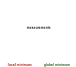
\includegraphics[width=\columnwidth]{figs/slam_local_min}
	\vspace*{-0.3in}
	\caption{An example of a local and global minimum for stereo SLAM with 10 poses and 20 landmarks from the ``Starry Night'' dataset. Ground-truth landmarks are shown as grey stars, ground-truth poses as blue frames, pose/landmark estimates are shown as frames/stars coloured red and green for local and global minima, respectively. Both minima are based on the same set of measurements: stereo pixel coordinates converted to Euclidean coordinates and relative-pose measurements. The local minimum was found via Gauss-Newton optimization ($\mbox{gradient}^2=8.87\times10^{-12}$, $\mbox{cost}=1.13\times10^3$) while the global minimum was found by solving an SDP tightened with \emph{redundant constraints} to obtain a rank-one solution ($\mbox{SVR}=2.43\times10^6$, $\mbox{cost}=9.36$). Top plot shows 3$\sigma$, anisotropic, uncertainty ellipsoids for measurements of the first pose.}
	\vspace*{-0.22in}
	\label{fig:slam_local_min}
\end{figure}

\IEEEPARstart{S}{tate-estimation} is an integral component of modern robotics systems. Workhorse algorithms for state-estimation -- such as localization and simultaneous localization and mapping (SLAM) -- are now capable of estimating hundreds of thousands of states on a single processor in real time \cite{rosenAdvancesInferenceRepresentation2021} and are far from the computational bottleneck of robotic systems. To obtain such levels of performance, these algorithms typically rely on local optimization methods (e.g., Gauss-Newton), which often exhibit super-linear convergence. In particular, SLAM has reached a high level of maturity in terms of both breadth and depth of understanding in the robotics community (see \cite{baileySimultaneousLocalizationMapping2006} and \cite{durrant-whyteSimultaneousLocalizationMapping2006} for a comprehensive review of SLAM).  

In recent years, we have seen a surge in interest in the use of convex, semidefinite relaxations to solve and certify the global optimality of robotic state-estimation and perception problems. 
In principle, these relaxations can be solved in polynomial time using interior-point methods\cite{vandenbergheSemidefiniteProgramming1996}. However, much of the interest in these algorithms is related to recent improvements in runtime, which have made certifiable methods more attractive for \emph{real-time} applications. These improvements have largely been brought to the robotics community by SE-Sync \cite{rosenSESyncCertifiablyCorrect2019}, which globally solves \emph{pose-graph optimization} (PGO) -- a cornerstone of modern SLAM algorithms -- by leveraging the low-rank nature of its semidefinite program (SDP) relaxation. A series of extensions to this method have been and continue to be developed \cite{rosenAdvancesInferenceRepresentation2021}.

Despite the success of these methods, they often rely on simplifying assumptions in order to apply these fast, low-rank algorithms. Perhaps most striking is the assumption of isotropic noise models that pervades the majority of the literature. Isotropic noise is often an unrealistic assumption for modern robotics, especially when more realistic sensor models are considered. For example, \cite{matthiesErrorModelingStereo1987} shows that conversion of stereo pixel coordinates to Euclidean coordinates yields noise distributions that should not be modeled isotropically. When the correct model is used, the resulting maximum-likelihood optimization includes \emph{matrix} (rather than \emph{scalar}) weighting factors. 

The introduction of matrix weighting in state-estimation problems with rotations typically leads to solution methods that are more involved. For example, though a closed-form, global solution exists for scalar-weighted Wahba's problem \cite{hornClosedformSolutionAbsolute1987, hornClosedFormSolutionAbsolute1988, wahbaLeastSquaresEstimate1965},\footnote{Wahba's problem can also be referred to as point-set registration.} when matrix weights are introduced, an iterative, local solver must be used \cite{chengTotalLeastSquaresEstimate2019, barfootStateEstimationRobotics2017}. Moreover, the introduction of matrix weights could lead to a cost function landscape that is less smooth, potentially resulting in more local minima. 

We will see that introduction of matrix weighting can also have a profound effect on the convex relaxations of state-estimation problems. In many cases, problems that have tight relaxations in the scalar-weighted case have a duality gap when matrix weighting is used. These relaxations can be \emph{tightened} by adding new constraints to the SDP, but the addition of these constraints precludes the application of the fast, low-rank optimization methods mentioned above. Therefore, it is paramount to understand the key causes of this loss of tightness.

In this paper, we explore the tightness of semidefinite relaxations of perception problems that have been generalized to include \emph{matrix weights} and expose the limitations that result from this generalization. We first introduce the requisite background on measurement models and semidefinite relaxation methods in Section \ref{Sec:Background}. In Section \ref{Sec:Formulations}, we explore the impact of matrix weighting on the formulation of two key state-estimation problems in robotics: localization and SLAM.
%In particular, we show that the introduction of matrix weighting necessarily changes the formulation of the semidefinite relaxation (compared to the scalar-weighted version \cite{holmesEfficientGlobalOptimality2023, iglesiasGlobalOptimalityPoint2020}). 
In Section \ref{Sec:Simulations}, we provide an in-depth, empirical study of the effects of matrix weighting, anisotropic noise, and stereo-camera measurements on the tightness of the semidefinite relaxations of Section \ref{Sec:Formulations}. We also evaluate these relaxations on a real-world dataset, both with and without redundant constraints in Section \ref{Sec:Dataset}. Finally, Section \ref{Sec:Conclusions} presents our conclusions and ideas for future research in this area.

\subsection{Related Work}

There is a large range of problems for which certifiable methods already exist. To name a few, methods for robust state estimation \cite{yangCertifiablyOptimalOutlierRobust2023,yangTEASERFastCertifiable2021}, sensor calibration \cite{wiseCertifiablyOptimalMonocular2020,giamouConvexIterationDistanceGeometric2022}, inverse kinematics \cite{giamouConvexIterationDistanceGeometric2022}, image segmentation \cite{huAcceleratedInferenceMarkov2019}, pose-graph optimization \cite{rosenSESyncCertifiablyCorrect2019}, multiple-point-set registration \cite{chaudhuryGlobalRegistrationMultiple2015, iglesiasGlobalOptimalityPoint2020}, range-only localization \cite{dumbgenSafeSmoothCertified2023}, and range-aided SLAM \cite{papaliaCertifiablyCorrectRangeAided2023} have all been explored. 

Many papers have considered the conditions under which a given problem \emph{can} be certified. In particular, \cite{cifuentesLocalStabilitySemidefinite2022} shows that, under certain technical conditions, problems that have zero duality gap when unperturbed (no noise) continue to enjoy zero duality gap as long as the perturbation parameter is within a bound (i.e., the underlying problem has sufficiently low noise). For state-estimation problems, this bound is often (but not always) found empirically to be larger than noise levels encountered in practice \cite{rosenSESyncCertifiablyCorrect2019, tianDistributedCertifiablyCorrect2021, erikssonRotationAveragingStrong2018}.

At present, certifiable perception problems can be broadly catagorized into two key groups: problems for which fast, low-rank solvers are available and problems that can be certified, but must still rely on slower SDP solution methods (e.g., interior-point methods). The next subsections provide more detail on each of these two groups.

\subsubsection{Fast Certifiable Perception}\label{Sec:FastPerception}

More so than other problems, global optimization of \emph{rotation synchronization} has been the subject of intense study in the vision community \cite{wilsonWhenRotationsAveraging2016, erikssonRotationAveragingStrong2018, brynteTightnessSemidefiniteRelaxations2022} and was one of the first to enjoy significant speed improvements by leveraging the \emph{low-rank} structure of the SDP relaxation via the so-called \emph{Riemannian Staircase} approach\cite{bandeiraTightnessMaximumLikelihood2017, boumalNonconvexBurerMonteiro2016}. 

Building off existing certification methods for PGO \cite{carloneLagrangianDuality3D2015} and inspired by the success of Riemannian methods for rotation-synchronization, \cite{rosenSESyncCertifiablyCorrect2019} introduced SE-Sync in the robotics community. SE-Sync solves PGO over $\mbox{SE}(d)$ by taking advantage of its \emph{separable} structure \cite{khosoussiSparseSeparableSLAM2016}, marginalizing the translation variables, and using the \emph{Riemannian Staircase} to solve the resulting rotation-synchronization problem. It was later shown that this technique could be used without marginalizing translations \cite{brialesCartanSyncFastGlobal2017} and extended to landmark-based SLAM \cite{holmesEfficientGlobalOptimality2023}, in both cases further exploiting problem sparsity. This method was also extended to a \emph{distributed} framework in \cite{tianDistributedCertifiablyCorrect2021} and has even been integrated into the recent Kimera-Multi pipeline \cite{tianKimeraMultiRobustDistributed2022}. Not surprisingly, these developments have inspired further advances in the original rotational synchronization problem \cite{dellaertShonanRotationAveraging2020}. 

Some of these methods boast runtimes that even rival state-of-the-art, local methods (e.g., Gauss-Newton-based methods \cite{gtsam}), with the added guarantee of a global certificate \cite{juricComparisonGraphOptimization2021, brialesCartanSyncFastGlobal2017}. An excellent review of the current state of certifiable methods is provided in \cite{rosenAdvancesInferenceRepresentation2021}.

\subsubsection{Certifiable Perception with Redundant Constraints}\label{Sec:RedundantConstraints}

Though SE-Sync and its derivatives are among the most performant algorithms in certifiable perception, there are several other certifiable perception problems to which fast, low-rank methods cannot yet be applied. In particular, this set of problems includes those whose semidefinite relaxations are not initially tight, but can be tightened through the addition of certain constraints. These constraints are to referred as \emph{redundant constraints} because they are redundant in the original formulation of the problem, but become nonredundant (and, indeed, linearly independent) in the lifted, semidefinite relaxation. The inability to use low-rank methods in this case is due to a technical condition that is violated by the introduction of these redundant constraints.\footnote{The low-rank, \emph{Burer-Monteiro} approach -- a building-block of many of these algorithms -- assumes Linear Independent Constraint Qualification of the original problem, which is violated by redundant constraints.}

This `tightening trick' has been known for some time in the optimization community \cite{nesterovSemidefiniteProgrammingRelaxations2000}, and has been applied to several problems \cite{ruizUsingRedundancyStrengthen2011, parriloSemidefiniteProgrammingRelaxations2003a}. In the computer-vision community, redundant constraints have been used to tighten generalized essential-matrix estimation \cite{zhaoCertifiablyGloballyOptimal2020}, relative-pose estimation between cameras \cite{garcia-salgueroTighterRelaxationRelative2022, brialesCertifiablyGloballyOptimal2018}, and registration using 3D primitives \cite{brialesConvexGlobal3D2017}. The formulation given in the latter paper is a degenerate version of our single-pose, matrix-weighted localization formulation (see Section \ref{Sec:Localization}), in which the use of (degenerate) matrix weights is motivated by geometry rather than noise distribution. 

Interestingly, both \cite{garcia-salgueroTighterRelaxationRelative2022} and \cite{brialesCertifiablyGloballyOptimal2018} showed that adding redundant constraints increases the level of measurement noise for which their respective problems remain tight. In the context of robotics, \cite{wiseCertifiablyOptimalMonocular2020} found a similar result when exploring the effect of redundant constraints on a sensor-calibration task. \cite{yangTEASERFastCertifiable2021} introduced redundant constraints in conjunction with \emph{graduated nonconvexity} \cite{yangGraduatedNonConvexityRobust2020} to solve \emph{robust} point-set registration globally. \cite{yangOneRingRule2020} and \cite{yangCertifiablyOptimalOutlierRobust2023} extended these results to several other robust perception problems by leveraging the Lasserre-moment hierarchy \cite{henrionMomentSOSHierarchyLectures2021,lasserreGlobalOptimizationPolynomials2001}. 

This hierarchy constitutes a powerful set of theoretical tools that are guaranteed to tighten the SDP relaxation of any \emph{polynomial} optimization problem through the use of redundant variables and constraints.\footnote{Note that this class of problems encompasses almost all of the certifiable perception problems to date.} The caveat to this method is that it requires the addition of new variables and constraints -- possibly \emph{ad infinitum} -- and can quickly become intractable in practice. Techniques such as \emph{Douglas-Rachford Splitting} for certification \cite{yangTEASERFastCertifiable2021} and the STRIDE algorithm \cite{yangCertifiablyOptimalOutlierRobust2023} have improved runtimes when the moment hierarchy is used, but are still far from real time. 

Since certification generally depends on the number of variables and constraints used, a more efficient tightening approach is to introduce only the minimal subset of variables and constraints required to make a given relaxation \emph{tight}, as is done in \cite{yangCertifiablyOptimalOutlierRobust2023}. This reflects the approach that we take in this paper, which is formalized in our concurrent work \cite{dumbgenGloballyOptimalState2023}.

\section{Background Material}\label{Sec:Background}

In this section, we provide the reader with some background material and notation that will be useful for the understanding of subsequent developments.

\subsection{Notation}\label{Sec:Notn}
We denote matrices with bold-faced, capitalized letters, $ \bm{A} $, column vectors with bold-faced, lower-case letters, $ \bm{a} $, and scalar quantities with normal-faced font, $ a $.
Let $ \mathbb{S}^n $ denote the space of $ n $-dimensional symmetric matrices and $ \mathbb{S}_+^n $ denote the space of $ n $-dimensional symmetric positive semidefinite matrices.
Let $ \|\cdot\|_F $ denote the Frobenius norm.
Let $ \diag{\bm{A}_1,\cdots,\bm{A}_N} $ denote the block-diagonal matrix with blocks corresponding to matrices $ \bm{A}_1,\cdots,\bm{A}_N $. Note that this includes the case where the $ \bm{A}_i $ are scalar (i.e., $\diag{a_1,\cdots,a_N}$, $a_i \in \mathbb{R}$).
Let $ \bm{I} $ denote the identity matrix, whose dimension will be clear from the context or otherwise specified.
Let $ \bm{0} $ denote the matrix with all-zero entries, whose dimension will be evident from the context.
Let the subscript ``$ 0 $'' denote the world frame.
Let $ \bm{t}_i^{ji} $ denote a vector from frame $ i $ to frame $ j $ expressed in frame $ i $ and $ \bm{C}_{ij} $ denote a rotation matrix that maps vectors expressed in frame $ j $ to equivalent vectors in frame $ i $.
Let $ \otimes $ denote the Kronecker product.
Let $ \vert S \vert $ denote the cardinality of the set $ S $.
Let $ \bm{A}^+ $ denote the Moore-Penrose pseudoinverse of a given matrix $ \bm{A} $.
Let $ \vect{\bm{A}} $ denote the vectorization (reshape) of a given matrix $ \bm{A} $.
Let $ (\cdot)^{\times} $ denote the linear, skew-symmetric operator as defined in \cite{barfootStateEstimationRobotics2017}.
Let $\left[N\right] = \left\{1,\cdots, N\right\} \subset \mathbb{N}$ be the set of indexing integers.



\subsection{Measurements Models}\label{Sec:MeasModels}

For 3D pose estimation problems, it is typical to represent the $i^{th}$ pose as a member of the Special Euclidean group:
\begin{equation}\label{eqn:pose_var}
	\mbox{SE}(3) = \left\{(\bm{C}_{i0}, \bm{t}_i^{i0})~:~\bm{C}_{i0}\in \mbox{SO}(3),~ \bm{t}_i^{i0}\in \mathbb{R}^3\right\}.
\end{equation}
In this paper, $\bm{C}_{i0}$ represents the rotation from the world frame to the $i^{th}$ pose frame and $\bm{t}_i^{i0}$ represents the translation vector from the world frame to the pose frame, expressed in the pose frame. Moreover, we will make use of the following \textit{homogeneous transformation} to represent a given robot pose:
\begin{equation}
	\bm{T}_{i0} = \begin{bmatrix}
		\bm{C}_{i0} & -\bm{t}_i^{i0} \\ \bm{0} & 1
	\end{bmatrix}.
\end{equation}
We adopt the \emph{factor graph} approach for our state-estimation problems (see \cite{dellaertFactorGraphsRobot2017} for an in-depth discussion of factor graphs). That is, we define a \textit{directed graph} or \emph{factor graph}, $ \Graph = \left(\VertSet, \EdgeSet\right)$, to keep track of existing measurements. The vertex set $ \VertSet = \VertSetP \cup \VertSetM $ is the union of the set of vertices representing poses, $ \VertSetP =\left[N_p\right]$, and the set of vertices representing landmarks, $ \VertSetM = \left[N_m\right]$. We assume that the edge set $\EdgeSet \subset \VertSet \times \VertSet$ is partitioned as $\EdgeSet= \EdgeSet_p \cup \EdgeSet_m$, where $\EdgeSet_p\subset \VertSet_p\times \VertSet_p$ represents relative-pose measurements and $\EdgeSet_m\subset \VertSet_p\times \VertSet_m$ represents measurements of a landmark from a given pose. We assume that each edge, $(i,j)\in \EdgeSet$, is associated with an error term, $\bm{e}_{ij}$, and a matrix weight, $\bm{W}_{ij}$.

Based on the graph $\Graph$, it can be shown that the \emph{maximum-a-posteriori} (MAP) estimate for the pose and landmark variables can be found via the minimization of the following cost function \cite{barfootStateEstimationRobotics2017}:
\begin{equation}\label{eqn:factor_graph}
	\begin{gathered}
		J = \sum\limits_{(i,k)\in\EdgeSet_p}  J_{ij}^{p} + \sum\limits_{(i,k)\in\EdgeSet_m} J_{ik}^{m}, \\ 
		J_{ij}^{p} = \bm{e}_{ij}^T \bm{W}_{ij} \bm{e}_{ij}, ~J_{ik}^{m} = \bm{e}_{ik}^T \bm{W}_{ik} \bm{e}_{ik},
	\end{gathered}
\end{equation}
where $J_{ij}^{p}$ and $J_{ik}^{m}$ are the cost `factors', with error terms, $\bm{e}_{ij}$ and $\bm{e}_{ik}$, that depend on the problem variables and weighting matrices, $\bm{W}_{ij}$ and $\bm{W}_{ik}$. The exact form of these terms are discussed in the next two sections. Though our formulation here is matrix-weighted in general, we focus on \emph{anisotropic} noise for pose-landmark measurements, with relative-pose measurements remaining \emph{isotropic}.

\subsubsection{Matrix-Weighted Pose-Landmark Measurements}\label{Sec:LandmarkMeas}

Each edge, $(i,k) \in \EdgeSet_m $, represents a measurement of the $k^{th}$ landmark from the $i^{th}$ pose. In robotics, the sensors that provide measurements of landmarks can often be modeled as
\begin{equation}
	\bm{d}_{ik} = \bm{g}(\bm{C}_{i0}\bm{m}_0^{k0} - \bm{t}_i^{i0}) + \bm{\epsilon}_{d,ik}, \quad \bm{\epsilon}_{d,ik} \in \mathcal{N}(\bm{0},\bm{\Sigma}_{d,ik}),
\end{equation}
where $ \bm{d}_{ik} $ represents the (raw) measurement of landmark $k$ from the $i^{th}$ pose variable, $\bm{m}_0^{k0}$ is the location of landmark $k$ in the global frame, $ \bm{g}(\cdot) $ is an invertible, smooth, nonlinear function, and $ \bm{\epsilon}_{d,ik} $ is a zero-mean error term having normal distribution with associated covariance matrix, $ \bm{\Sigma}_{d,ik} $. 

It is often desirable to convert measurements $ \bm{d}_{ik} $ to a more convenient form by inverting the measurement model (if possible) and defining 
\begin{align}
	\tilde{\bm{m}}_i^{ki} &= \bm{g}^{-1}(\bm{d}_{ik})\in \mathbb{R}^3 \nonumber\\
	&=\bm{T}_{i0} \left[\bm{m}_0^{k0^T} ~ 1\right]^T + \bm{\epsilon}_{ik}\nonumber\\
	&= \bm{C}_{i0}\bm{m}_0^{k0} - \bm{t}_i^{i0} + \bm{\epsilon}_{ik},
\end{align}
where $\bm{\epsilon}_{ik} $ represents approximately Gaussian, zero-mean noise. Regardless of whether $ \bm{\Sigma}_{d,ik} $ represents isotropic noise, the (linearly-transformed) covariance of $\bm{\epsilon}_{ik} $ is typically \textit{anisotropic} and is given by
\begin{equation}
	\bm{\Sigma}_{ik} = \bm{G}^T \bm{\Sigma}_{d,ik} \bm{G},
\end{equation}
where $\bm{G}$ is the Jacobian of the inverse measurement function $\bm{g}^{-1}(\cdot)$ \cite{matthiesErrorModelingStereo1987}. The associated error term for this measurement factor becomes
\begin{equation}\label{eqn:lm_error_term}
	\bm{e}_{ik} = \tilde{\bm{m}}_i^{ki} - \bm{C}_{i0}\bm{m}_0^{k0} - \bm{t}_i^{i0}.
\end{equation}
The weighting matrix in the cost factor in the MAP estimation, \eqref{eqn:factor_graph}, is then given by the inverse of the covariance matrix, $ \bm{W}_{ik} = \bm{\Sigma}^{-1}_{ik} $. Note that solving the problem under the simplifying assumption of isotropic noise -- that is, $ \bm{W}_{ik} = \sigma_{ik} \bm{I}$ with $ \sigma_k \in \mathbb{R}$ -- can be extremely detrimental to the quality of the final solution \cite{matthiesErrorModelingStereo1987}. 

A key example of such a situation arises in a common preprocessing step of stereo-vision problems, in which pixel and disparity measurements are converted to Euclidean point measurements by inverting a known camera model.  It has been shown that this results in measurement uncertainty that is much larger in the depth direction of a given camera pose \cite{matthiesErrorModelingStereo1987,barfootPoseEstimationUsing2011} (c.f. Figure \ref{fig:slam_local_min}). A derivation of the inverse stereo measurement model and associated covariance is provided in the Supplementary Material \ref{SM:stereo}. 

\subsubsection{Relative-Pose Measurements}\label{Sec:RelPoseMeas}

Each edge, $(i,j) \in \EdgeSet_p $, represents a relative-pose measurement, which can be expressed as the homogeneous transformation,
\begin{equation}
	\tilde{\bm{T}}_{ij} = \begin{bmatrix}
		\tilde{\bm{C}}_{ij} & \tilde{\bm{t}}_i^{ji} \\ \bm{0} & 1
	\end{bmatrix}.
\end{equation}
%It is generally assumed that these measurements are perturbed by noise with a known distribution. For example, \cite{carlone2015lagrangian} and \cite{rosenSESyncCertifiablyCorrect2019} (among others) assume the following (isotropic) noise model when solving pose-graph optimization:
%\begin{equation*}
%	\begin{array}{lr}
%		\tilde{\bm{t}}_i^{ji} = \bm{C}_{i0}\bm{C}_{j0}^T\bm{t}_j^{j0} - \bm{t}_i^{i0} + \bm{\epsilon}_t,& \bm{\epsilon}_t \sim \mathcal{N}(\bm{0}, \tau_{ij}^2\bm{I}), \\
%		\tilde{\bm{C}}_{ij} = \bm{C}_{j0}\bm{C}_{i0}^T\tilde{\bm{C}}, &\tilde{\bm{C}} \sim \mathcal{L}(\bm{I}, \sigma_{ij}^2),
%	\end{array}
%\end{equation*}
%where $\mathcal{N}(\bm{\mu},\bm{\Sigma})$ is the Gaussian distribution and $\mathcal{L}(\bm{M},\sigma)$ is the Langevin distribution over $\mbox{SO}(3)$ with mode $\bm{M}$ and concentration parameter $\sigma$. These choices of error distribution lead naturally to \textit{scalar-weighted} factors in the estimation cost function via the standard log-likelihood argument. 

In a robotics context, these relative-pose measurements often represent IMU-based measurement information, dynamics-based prior belief propagation, or aggregate measurement data between keyframes. Similarly to \cite{brialesCartanSyncFastGlobal2017}, we define the following relative-pose error term:
\begin{equation}\label{eqn:rel_pose_err}
	\bm{e}_{ij} = \vect{\tilde{\bm{T}}_{ij}\bm{T}_{j0} - \bm{T}_{i0}}.
\end{equation}
This relative-pose error allows for the addition of \emph{prior} information about the pose variables to \eqref{eqn:factor_graph}. In this case, the relative-pose error is defined with respect to the `world' frame (index $0$):
\begin{equation}\label{eqn:prior_pose_err}
	\bm{e}_{0j} = \vect{\tilde{\bm{T}}_{0j}\bm{T}_{j0} - \bm{I}}.
\end{equation}
Though $\bm{W}_{ij} \succeq \bm{0} $ can be an \emph{arbitrary}, positive semidefinite matrix, we select weight matrices of the form $\bm{W}_{ij}=\diag{\sigma^2_{ij},\sigma^2_{ij},\sigma^2_{ij},\tau^2_{ij}}^{-1} \otimes \bm{I}$, since it allows us to express our cost factor as
\begin{equation}\label{eqn:rel_pose_cost}
	J_{ij} = \frac{1}{\sigma^2_{ij}} \left\Vert \tilde{\bm{C}}_{ij}\bm{C}_{j0} - \bm{C}_{i0}\right\Vert_F^2 + \frac{1}{\tau^2_{ij}} \left\Vert \tilde{\bm{t}}^{ji}_{i} - \tilde{\bm{C}}_{ij}\bm{t}_j^{j0} + \bm{t}_i^{i0} \right\Vert_2^2,
\end{equation}
where $\sigma_{ij}$ and $\tau_{ij}$ are scalar weights. This form of cost factor is similar to the cost used in pose-graph optimization problems (c.f. \cite{brialesCartanSyncFastGlobal2017, rosenSESyncCertifiablyCorrect2019, holmesEfficientGlobalOptimality2023}), but is quadratic for our choice of pose variables, \eqref{eqn:pose_var}.\footnote{The choice to represent translation variables in the \emph{local} frame ($\bm{t}_i^{i0}$) rather in the \emph{world} frame ($\bm{t}_0^{i0}$) led to tighter relaxations in our preliminary analyses.}

\subsection{Convex Relaxations of QCQPs}\label{Sec:Relaxation}

We review the well-known procedure for deriving convex, SDP relaxations of a standard form of polynomial optimization problem. This procedure was pioneered in \cite{shorQuadraticOptimizationProblems1987} and has become the cornerstone of \textit{certifiably correct methods} in robotics and computer vision \cite{rosenAdvancesInferenceRepresentation2021,brynteTightnessSemidefiniteRelaxations2022}. Here we consider a \textit{homogeneous}, \textit{quadratically constrained quadratic problem} (QCQP) expressed in the following standard form:
\begin{equation}\label{opt:QCQP}
	\min\limits_{\bm{z}} \left\{ \bm{z}^T\bm{Q}\bm{z} ~\vert~ \bm{z}^T\bm{A}_i\bm{z} = 0,\forall i \in \indset{N_c}, \bm{z}^T\bm{A}_0\bm{z} = 1 \right\},
\end{equation}
where $ \bm{z}\in\mathbb{R}^n $ is the homogeneous optimization variable, $ \bm{Q}\in\mathbb{R}^{n\times n} $ represents the quadratic cost, the $ \bm{A}_i $ correspond to $ N_c $ quadratic constraints, and $ \bm{A}_0 $ corresponds to the so-called \emph{homogenizing constraint}\cite{cifuentesLocalStabilitySemidefinite2022}. Note that any problem with quadratic cost and constraints can be converted into a problem of this form \cite{cifuentesLocalStabilitySemidefinite2022}.

In general, problems with quadratic equality constraints, such as QCQPs, are difficult to solve optimally because they are nonconvex \cite{boydConvexOptimization2004}. However, a popular approach to obtaining globally optimal solutions to QCQPs involves first deriving the Lagrangian dual problem and then showing that \textit{strong duality} holds at a given solution (see \cite{boydConvexOptimization2004} for details of these concepts). 
%Furthermore, the development given in \cite{cifuentesLocalStabilitySemidefinite2022} allows to study the conditions under which strong duality will hold \emph{a priori} for a given problem.

The Lagrangian of Problem \eqref{opt:QCQP} is given by,
\begin{equation}\label{eqn:Lagrangian}
	\mathcal{L}(\bm{z},\bm{\lambda}, \rho) = \bm{z}^T\left(\bm{Q} + \rho\bm{A}_0 +\sum\limits_{i=1}^{N_c} \lambda_i \bm{A}_i\right) \bm{z} - \rho,
\end{equation}
where $ \rho $ and $ \bm{\lambda} = \left[\lambda_1~\cdots~\lambda_{N_c}\right]^T $ are the Lagrange multipliers corresponding to the simple homogenizing and the $N_c$ quadratic constraints, respectively.
Using the Lagrangian, we can define the (convex) dual of Problem \eqref{opt:QCQP} as follows:
\begin{equation}\label{opt:Dual}
	\begin{array}{rl}
		d^*=\max\limits_{\bm{H},\bm{\lambda},\bm{\rho}} &-\rho \\ 
		s.t. & \bm{H} = \bm{Q} + \rho\bm{A}_0 +\sum\limits_{i=1}^{N_c} \lambda_i \bm{A}_i, \\
		& \bm{H} \succeq \bm{0}.
	\end{array}
\end{equation}
Note that the positive semidefinite condition is required to ensure that the minimization of the Lagrangian over $ \bm{z} $ is finite in \eqref{eqn:Lagrangian}. Now, we can also compute the dual of Problem \eqref{opt:Dual}, yielding an SDP relaxation of the original QCQP:
\begin{equation}\label{opt:SDP}
	\begin{array}{rl}
		\min\limits_{\bm{Z}} & \inner{\bm{Q}}{\bm{Z}}\\
		s.t.&\inner{\bm{A}_i}{\bm{Z}}= 0, \quad i = \left[N_c\right]\\
		& \inner{\bm{A}_0}{\bm{Z}}= 1, \\
		& \bm{Z} \succeq \bm{0}.
	\end{array}
\end{equation}
It is well known that if the optimal solution $ \bm{Z}^* $ satisfies $ \rank{\bm{Z}^*}=1 $ then the convex relaxation is \textit{tight} to the original QCQP.\footnote{Indeed, the addition of a constraint enforcing this condition to Problem \eqref{opt:SDP} would render it equivalent to Problem \eqref{opt:QCQP}, but the resulting optimization problem would be nonconvex.} In addition, this condition implies that the solution can be factorized as $ \bm{Z}^* = \bm{z}^* \bm{z}^{*T} $, where $ \bm{z}^* $ is the \textit{globally optimal} solution of Problem \eqref{opt:QCQP}. This result has been proved rigorously by \cite{cifuentesLocalStabilitySemidefinite2022}, among others, and depends on the inherent properties of the QCQP formulation and the fact that strong duality holds \emph{generically} for SDPs.\footnote{This is subject to the usual requirement of constraint qualification.}

This development provides two means of obtaining the globally optimal solutions to the QCQP:
\begin{enumerate}
	\item We can solve Problem \eqref{opt:SDP} directly and verify (numerically) that the rank of the optimal solution, $ \bm{Z}^* $, is equal to one. The factorization $ \bm{Z}^* = \bm{z}^* \bm{z}^{*T} $ yields the globally optimal solution, $ \bm{z}^* $, to the QCQP.
	\item Given a candidate solution, $ \hat{\bm{z}} $, found via a fast, local-optimization method, we can determine the corresponding \textit{unique} Lagrange multipliers, $ \rho $ and $ \bm{\lambda} $, via first-order optimality conditions. Finally, if $ \bm{H} $ is positive semidefinite, then we have a \textit{certificate} of global optimality. For this reason, we refer to $ \bm{H} $ as the \textit{certificate} matrix.
\end{enumerate}
The first approach involves directly solving an SDP, which, in general, can be done in \textit{polynomial time} using interior-point methods \cite{vandenbergheSemidefiniteProgramming1996}. These methods are fast for small problems and even tractable for problems of up to thousands of variables, but become prohibitive for the larger problems often seen in robotics. Therefore, many recent, state-of-the-art methods leverage low-rank SDP techniques such as that of \emph{Burer and Monteiro} \cite{burerNonlinearProgrammingAlgorithm2003a} and the \emph{Riemannian Staircase} \cite{rosenSESyncCertifiablyCorrect2019, boumalNonconvexBurerMonteiro2016} to solve larger problem instances in real time. These have become the default approach for many certifiably optimal problems in robotics and computer vision. However, these fast methods often require a \emph{certification} step via the second approach.

Especially when the problem dimension is large, the bottleneck of the second approach typically lies in determining the minimum eigenvalues of $ \bm{H} $ \cite{rosenAcceleratingCertifiableEstimation2022}. However, in particular problems where $ \bm{H} $ is sparse, iterative eigenvalue methods can greatly improve the runtime for this task and have become the \emph{de facto} certification technique \cite{rosenComputationalEnhancementsCertifiably2017, rosenAcceleratingCertifiableEstimation2022}. 

Additionally, if it is known \textit{a priori} that strong duality holds for a given problem, then failure of the certification test in the second method indicates that the candidate solution, $ \hat{\bm{z}}$, is exactly a \textit{local minimum}. Such \textit{a priori} proofs as well as empirical evidence suggest that tightness depends on the level of noise in a problem instance \cite{cifuentesLocalStabilitySemidefinite2022, rosenSESyncCertifiablyCorrect2019, holmesEfficientGlobalOptimality2023,  wiseCertifiablyOptimalMonocular2020, iglesiasGlobalOptimalityPoint2020}. 

We once again stress that when redundant constraints are used to tighten SDP relaxations, these low-rank, fast SDP relaxation techniques are precluded.\footnote{This is due, in part, to a technical assumption in the Burer-Monteiro method that has not yet been fully explored in the literature. It may yet be possible to use these methods even with redundant constraints.} The use of redundant constraints also prevents fast certification of minima found via local methods, since the Lagrange multipliers, $ \bm{\lambda} $, are no longer uniquely determined by the first-order optimality conditions. In this case, certification effectively amounts to solving an SDP via interior-point methods, though there has been some success in applying methods such as \textit{Douglas-Rachford Splitting} \cite{yangTEASERFastCertifiable2021}. As a result, the use of redundant constraints for medium-to-large perception problems leads to runtimes that are currently prohibitive for real-time application.

Therefore, establishing a `threshold' below which redundant constraints are \emph{not} necessary is crucial for distinguishing the robotics problems that can be globally solved in realtime via state-of-the-art techniques. Indeed, a goal of this paper is to determine this threshold for estimation problems that involve matrix weights.

\section{Problem Formulations}\label{Sec:Formulations}

In this section, we provide QCQP formulations for the matrix-weighted localization and SLAM problems that are considered herein. We demonstrate how the costs can be formulated in the standard quadratic form of Problem \eqref{opt:QCQP}. In the interest of brevity, we do not explicitly show the conversion of the constraints into the standard form.

\subsection{Matrix-Weighted Localization}\label{Sec:Localization}

In this section, we consider localization problems with matrix weights. That is, we consider the problem of determining the estimate of a sequence of poses given matrix-weighted measurements of a set of \emph{known} landmarks. We assume that point correspondences are known and correct. 

The maximum-likelihood estimate of the poses is given by the solution to the following least-squares optimization problem:
\begin{equation}
	\label{opt:Localize}
	\begin{array}{rl}
		\min\limits_{\bm{C}_{i0},\bm{t}_i^{i0}, \forall  i \in \VertSetP} &\sum\limits_{(i,k)\in\EdgeSet_m} \bm{e}_{ik}^T \bm{W}_{ik} \bm{e}_{ik} \\
		\mbox{s.t.} &\bm{C}_{i0}\in\mbox{O}(3),~\forall i = \VertSetP, \\
		\mbox{where} & \bm{e}_{ik} = \tilde{\bm{m}}_i^{ki} - \bm{C}_{i0}\bm{m}_0^{k0} + \bm{t}_i^{i0} ,
	\end{array}
\end{equation}
where the variable definitions are consistent with those provided in Section \ref{Sec:MeasModels}. 

It should be noted that we have relaxed the \textit{special orthogonal group} membership constraints of the pose rotations ($\bm{C}_{i0}\in\mbox{SO}(3)$) to membership in the orthogonal group ($\bm{C}_{i0}\in\mbox{O}(3)$). This relaxation is fairly common for problems involving rotation matrices, since membership in the \textit{special orthogonal group} requires a \emph{cubic} constraint \cite{brialesConvexGlobal3D2017}. In some cases, it has been shown empirically that this relaxation does not affect the tightness of subsequent convex relaxations (c.f. \cite{rosenSESyncCertifiablyCorrect2019, erikssonRotationAveragingStrong2018, iglesiasGlobalOptimalityPoint2020, holmesEfficientGlobalOptimality2023}). However, there are some instances in which this relaxation \emph{does} affect tightness \cite{wiseCertifiablyOptimalMonocular2020, brialesConvexGlobal3D2017}. It is interesting to note that both of these latter cases leveraged redundant constraints to tighten their respective problems.\footnote{An additional distinction of these latter problems is that both involved \emph{vectorized} rotation variables, which lead to relaxations with higher degrees of freedom than if the variables are represented in matrix form, as in \cite{rosenSESyncCertifiablyCorrect2019,brialesCartanSyncFastGlobal2017}.}

It is immediately clear that this problem is separable in each set of pose variables, since there are no constraints or cost elements linking any two poses. Therefore, the problem may be divided into $N_p$ subproblems, each being equivalent to the matrix-weighted version of Wahba's problem \cite{chengTotalLeastSquaresEstimate2019, wahbaLeastSquaresEstimate1965}. In the scalar-weighted case ($ \bm{W}_{ik} = w_{ik} \bm{I} $), there is a closed-form, global solution to Wahba's problem \cite{hornClosedFormSolutionAbsolute1988}. However, for the general matrix-weighted case, a key simplification of the cost function is no longer possible and solutions must be found iteratively with no guarantee of global optimality \cite{barfootPoseEstimationUsing2011,barfootStateEstimationRobotics2017, crassidisSurveyNonlinearAttitude2007}.  However, this problem is clearly a QCQP: $\bm{e}_{ik}$ is \emph{linear} in $\bm{C}_{i0}$ and $\bm{t}_i^{i0}$, and the $\mbox{O}(3)$ constraints are quadratic. 

We now demonstrate how the cost of Problem \eqref{opt:Localize} can be cast into the standard QCQP form given in \ref{Sec:Relaxation}. Consider a single element of the sum over edges in $\EdgeSet_m $ in the cost function:
\begin{align*}
	J_{ik}=&(\tilde{\bm{m}}_i^{ki} - \bm{C}_{i0}\bm{m}_0^{k0} + \bm{t}_i^{i0})^T \bm{W}_k (\tilde{\bm{m}}_i^{ki} - \bm{C}_{i0}\bm{m}_0^{k0} + \bm{t}_i^{i0}) \\
	=& \tilde{\bm{m}}_i^{ki^T}\bm{W}_k\tilde{\bm{m}}_i^{ki} w^2 - 2 w\tilde{\bm{m}}_i^{ki^T}\bm{W}_k\bm{C}_{i0}\bm{m}_0^{k0}  \\
	&+ 2 w\tilde{\bm{m}}_i^{ki^T}\bm{W}_k\bm{t}_i^{i0} -2\bm{m}_0^{k0^T}\bm{C}_{i0}^T\bm{W}_k\bm{t}_i^{i0}\\
	& + \bm{m}_0^{k0^T}\bm{C}_{i0}^T\bm{W}_k\bm{C}_{i0}\bm{m}_0^{k0} + \bm{t}_i^{i0^T}\bm{W}_k\bm{t}_i^{i0},
\end{align*}
where we introduce a so-called \textit{homogenizing variable}, $ w $, which is subject to the \textit{homogenizing constraint}, $ w^2 = 1 $ \cite{wiseCertifiablyOptimalMonocular2020, cifuentesLocalStabilitySemidefinite2022}. We collect the relevant optimization variables into a single vector, $ \bm{x}_i^T = \begin{bmatrix} \bm{c}_{i0}^T &  \bm{t}_i^{i0^T}& w \end{bmatrix} $, where $ \bm{c}_{i0}=\vect{\bm{C}_{i0}} $, which allows us to re-express the cost element as
\begin{equation}
	J_{ik}= \bm{x}_i^T\bm{Q}_{ik}\bm{x}_i,
\end{equation}
where the symmetric cost matrix, $\bm{Q}_{ik}$, is given by	
\begin{equation*}
	\resizebox{0.98\columnwidth}{!}{$\begin{bmatrix}
			\bm{m}_0^{k0}\bm{m}_0^{k0^T} \otimes \bm{W}_k  & -\bm{m}_0^{k0}\otimes\bm{W}_k & -\bm{m}_0^{k0}\otimes\bm{W}_k\tilde{\bm{m}}_i^{ki}\\
			 -\bm{m}_0^{k0^T}\otimes\bm{W}_k & \bm{W}_k & -\bm{W}_k\tilde{\bm{m}}_i^{ki} \\
			-\bm{m}_0^{k0^T}\otimes\tilde{\bm{m}}_i^{ki^T}\bm{W}_k & -\tilde{\bm{m}}_i^{ki^T}\bm{W}_k & \tilde{\bm{m}}_i^{ki^T}\bm{W}_k\tilde{\bm{m}}_i^{ki}
		\end{bmatrix}.$}
\end{equation*}

We used the facts that $ \tr{\bm{A}\bm{B}\bm{C}} = (\bm{C}^T\otimes\bm{A}) \vect{\bm{B}}$, $ \bm{A} = 1\otimes\bm{A} $, and $ (\bm{A}\otimes\bm{B})(\bm{C}\otimes\bm{D}) = (\bm{AC}\otimes\bm{BD}) $\cite{magnusMatrixDifferentialCalculus2019}. 

It is straightforward to show that the full cost of Problem \eqref{opt:Localize} can be constructed by permuting and summing the matrices, $\bm{Q}_{ik}$, according to edges in $\EdgeSet_m$ and a given pose variable ordering:\footnote{Alternate variable choices are possible here (c.f. \cite{brialesCartanSyncFastGlobal2017,tianDistributedCertifiablyCorrect2021}), but we select this `vectorized' form because it simplifies the study of SDP tightness.}
\begin{equation}
	\bm{z}^T = \begin{bmatrix}
		\bm{c}_{10}^T & \bm{t}_1^{10^T} & \cdots &  \bm{c}_{N_p 0}^T & \bm{t}_{N_p}^{N_p0^T} & w
	\end{bmatrix}.
\end{equation}

The single-pose version of this problem admits a convex semidefinite relaxation that was explored in \cite{brialesConvexGlobal3D2017} and \cite{olssonSolvingQuadraticallyConstrained2008} with the motivation of representing different geometric primitive measurements (lines and planes), rather than anisotropic noise. It was found that the addition of a few key redundant constraints made the relaxation tight even when noise levels were high. Since this problem is small in dimension, its SDP relaxation can be solved quickly using modern interior-point solvers and the addition of redundant constraints will not increase the solution time considerably. However, as we will see in the next section, this is no longer the case when relative-pose measurements are introduced.

In the Supplementary Material \ref{SM:SDPStability}, we prove that Problem \eqref{opt:Localize} is always tight when measurement noise levels are low enough and the weighting matrices are non-degenerate.

\subsection{Matrix-Weighted Localization with Relative-Pose Measurements}

We now consider the effect of introducing \textit{relative-pose measurements} described in Section \ref{Sec:RelPoseMeas}. Adding the associated cost factors to Problem \eqref{opt:Localize}, we define the matrix-weighted localization problem with relative-pose measurements:
\begin{equation}
	\label{opt:LocalizeRelPose}
	\hspace*{-10pt}\begin{array}{rl}
		\min\limits_{\bm{C}_{i0},\bm{t}_i^{i0}, \forall  i \in \VertSetP} &\sum\limits_{(i,k)\in\EdgeSet_m} \bm{e}_{ik}^T \bm{W}_{ik} \bm{e}_{ik} +\sum\limits_{(i,j)\in\EdgeSet_p}  \bm{e}_{ij}^T \bm{W}_{ij} \bm{e}_{ij}\\
		\mbox{where} & \bm{e}_{ik} = \tilde{\bm{m}}_i^{ki} - \bm{C}_{i0}\bm{m}_0^{k0} + \bm{t}_i^{i0} , \\
		&\bm{e}_{ij} = \vect{\tilde{\bm{T}}_{ij}\bm{T}_{j0} - \bm{T}_{i0}}, \\
		\mbox{s.t.} &\bm{C}_{i0}^T \bm{C}_{i0} = \bm{I},~\forall i \in \VertSetP. \\
	\end{array}
\end{equation}
We have shown in the previous section how the pose-landmark cost factors can be expressed in the form of Problem \eqref{opt:QCQP}. It remains to show that the same is possible for the relative-pose cost factors, \eqref{eqn:rel_pose_cost}. Each edge in $\EdgeSet_p$ represents a cost element of the following form:
\begin{equation}
	J_{ij} = \frac{1}{\sigma^2_{ij}} \left\Vert \tilde{\bm{C}}_{ij}\bm{C}_{j0} - \bm{C}_{i0}\right\Vert_F^2 + \frac{1}{\tau^2_{ij}} \left\Vert \tilde{\bm{t}}^{ji}_{i} - \tilde{\bm{C}}_{ij}\bm{t}_j^{j0} + \bm{t}_i^{i0} \right\Vert_2^2.
\end{equation}
As before, we collect the relevant variables,
\begin{equation*}
	\bm{x}_{ij}^T = \begin{bmatrix} \bm{c}_{i0}^T&\bm{c}_{j0}^T  & \bm{t}_i^{i0^T} & \bm{t}_j^{j0^T} & w\end{bmatrix},
\end{equation*}
allowing us to write the cost element as
\begin{gather*}
	J_{ij}= \bm{x}_{ij}^T\bm{Q}_{ij}\bm{x}_{ij}, \\
	\bm{Q}_{ij} = \begin{bmatrix}
		\frac{1}{\sigma^2_{ij}}\bm{Q}_{r,ij} & \bm{0}\\
		\bm{0}&\frac{1}{\tau^2_{ij}}\bm{Q}_{t,ij}
	\end{bmatrix},
\end{gather*}
with
\begin{gather*}
	\bm{Q}_{r,ij}=\begin{bmatrix}
		\bm{I}  &  -\bm{I}\otimes\tilde{\bm{C}}_{ij}^T\\
		-\bm{I}\otimes\tilde{\bm{C}}_{ij} & \bm{I}
	\end{bmatrix}, \\ 
	\bm{Q}_{t,ij}=\begin{bmatrix}
		\bm{I}  &  -\tilde{\bm{C}}_{ij} & \tilde{\bm{t}}_{i}^{ji}\\
		-\tilde{\bm{C}}_{ij}^T & \bm{I} & -\tilde{\bm{C}}_{ij}\tilde{\bm{t}}_{i}^{ji}\\
		\tilde{\bm{t}}_{i}^{ji^T} &  -\tilde{\bm{t}}_{i}^{ji^T}\tilde{\bm{C}}_{ij}^T & \tilde{\bm{t}}_{i}^{ji^T} \tilde{\bm{t}}_{i}^{ji}
	\end{bmatrix}.
\end{gather*}

As before, the cost of Problem \eqref{opt:LocalizeRelPose} can now be expressed in the standard form by permuting and summing the cost matrices according to a prescribed variable ordering. However, Problem \eqref{opt:LocalizeRelPose} is no longer separable in terms of pose variables, meaning that directly solving the SDP relaxation becomes much slower for reasonably sized problems (e.g., $N_p \geq 20$).

As we will show in Section \ref{Sec:NoiseAnalysis}, in some problem instances the level of noise can break the tightness of the convex relaxation. This tightness can be maintained by adding the following redundant constraints:
\begin{subequations}\label{eqn:so3_constraints}
	\begin{flalign}
		\bm{C}_{i0} \bm{C}_{i0}^T - \bm{I} = \bm{0},
	\end{flalign}
	\vspace*{-20pt}
	\begin{flalign}
		(\bm{c}_{i0}^{j})^\times\bm{c}_{i0}^{k} - \bm{c}_{i0}^{l} = \bm{0}, ~\forall (j,k,l)\in \mbox{cyclic}(1,2,3),
	\end{flalign}
	\vspace*{-20pt}
	\begin{flalign}
		\bm{c}_{i0}^{j^T}\bm{c}_{i0}^{j} - \bm{r}_{i0}^{k^T}\bm{r}_{i0}^{k} = \bm{0}, ~\forall j,k\in \left\{1,2,3\right\},
	\end{flalign}
\end{subequations}
where $\bm{c}_{i0}^{j}$ and $\bm{r}_{i0}^{k}$ represent the $j^{th}$ column and $k^{th}$ row of $\bm{C}_{i0}$, respectively, and $\mbox{cyclic}()$ denotes the cyclic group. Note that the first two redundant constraints were also necessary in \cite{brialesConvexGlobal3D2017} and \cite{wiseCertifiablyOptimalMonocular2020}. However, these additional constraints then preclude the use of the fast solvers mentioned in Section \ref{Sec:Relaxation}. Therefore, it is very important to characterize the noise regime for which the convex relaxation of Problem \eqref{opt:LocalizeRelPose} is still tight, which is the subject of Section \ref{Sec:NoiseAnalysis}.

\subsection{Matrix-Weighted Landmark-based SLAM}

In this section, we explore the effect of matrix weighting when the landmark locations, $\bm{m}_0^{k0}$, in Problem \eqref{opt:LocalizeRelPose} are not known \emph{a priori}. The convex relaxation of this problem, known as landmark-based SLAM, has already been studied in the \emph{scalar-weighted} context \cite{holmesEfficientGlobalOptimality2023} and was generally found to be tight for noise levels well above those found in practical robotics scenarios. 

Note that since the error term in \eqref{eqn:lm_error_term} is now quadratic in its variables, the cost function of Problem \eqref{opt:LocalizeRelPose} becomes \emph{quartic}. In the scalar-weighted case ($\bm{W}_{ik} = w_{ik}\bm{I}$), this issue is obviated by premultiplying the error terms by the inverse pose rotations to regain \emph{quadratic} cost factors:
\begin{align*}
	J_{ik} &= \bm{e}_{ik}^T \bm{W}_{ik}\bm{e}_{ik} \\
	&= (\bm{C}_{i0}^T\bm{e}_{ik})^T \bm{C}_{i0}^T\bm{W}_{ik}\bm{C}_{i0} (\bm{C}_{i0}^T\bm{e}_{ik})\\
	&= w_{ik}(\bm{C}_{i0}^T\bm{e}_{ik})^T (\bm{C}_{i0}^T\bm{e}_{ik}), \\ 
	\bm{C}_{i0}^T\bm{e}_{ik} &= \bm{C}_{i0}^T\tilde{\bm{m}}_i^{ki} - (\bm{m}_0^{k0} - \bm{t}_0^{i0}).
\end{align*}
However, in the matrix-weighted case, this simplification is not possible because, in general, $\bm{C}_{i0}^T\bm{W}_{ik}\bm{C}_{i0}\neq \bm{W}_{ik}$. This reflects the fact that the measurement noise \emph{has an orientation} and depends on the (unknown) observation frame.\footnote{This would not be an issue if all measurements were defined in a common frame, but, in practice, measurements are always taken in the robot's frame of reference.} 

In order to cast Problem \eqref{opt:LocalizeRelPose} as a QCQP, we follow a similar strategy to \cite{dumbgenSafeSmoothCertified2023} and \cite{brialesCertifiablyGloballyOptimal2018} by introducing \textit{substitution variables}, $ \bm{m}_i^{ki} $, corresponding to each available measurement, $ \tilde{\bm{m}}_i^{ki} $. These new variables must satisfy the following (quadratic) constraints:
\begin{equation}
	\bm{m}_i^{ki} = \bm{C}_{i0}	\bm{m}_0^{k0} - \bm{t}_i^{i0}, \quad \forall (i,k)\in\EdgeSet_m.
\end{equation}

When the landmarks become unknown, a gauge freedom is also introduced into the problem. This has an important implication for the SDP solution; the well-known SLAM gauge freedom results in solution symmetries that cause the rank of the SDP solution to be higher than one, even when it is numerically tight \cite{brialesCertifiablyGloballyOptimal2018}. To fix this freedom, we assume that a \emph{prior} factor term is included in the pose-graph terms for at least one pose.\footnote{As with SLAM problems in general, the pose variable in the prior, $\tilde{\bm{T}}_{j0}$, is typically used to `lock' the solution to a known pose using some exteroceptive measurement, such as GPS. However, for our purposes it can be set arbitrarily without loss of generality.}

The optimization can now be written as
\begin{equation}
	\hspace*{-5pt}
	\label{opt:SLAM}
	\begin{array}{rl} 
		\min \limits_{ \substack{\bm{C}_{i0},\bm{t}_i^{i0}, \\ \bm{m}_0^{k0},\bm{m}_i^{ki} \\ \forall i\in \VertSetP,~ \forall k\in\VertSetM } } & \hspace*{-20pt}\sum\limits_{(i,k)\in\EdgeSet_m} \bm{e}_{ik}^T \bm{W}_{ik} \bm{e}_{ik} + \hspace*{-7pt}\sum\limits_{(i,j)\in\EdgeSet_p}  \bm{e}_{ij}^T \bm{W}_{ij} \bm{e}_{ij}\hfill \\
		\mbox{where} & \bm{e}_{ik} = \tilde{\bm{m}}_i^{ki} - \bm{m}_i^{ki},\\
		&\bm{e}_{ij} = \vect{\tilde{\bm{T}}_{ij}\bm{T}_{j0} - \bm{T}_{i0}},\\
		\mbox{s.t.}&\bm{C}_{i0}\in\mbox{O}(3), \quad\forall i = \VertSetP,\\
		& \bm{m}_i^{ki} = \bm{C}_{i0}\bm{m}_0^{k0} - \bm{t}_i^{i0}, \quad \forall (i,k)\in\EdgeSet_m.
	\end{array}
\end{equation}
It is straightforward to show that the pose-landmark cost elements can now be written in the standard form:
\begin{equation*}
	J_{ik}=\begin{bmatrix}
		\bm{m}_i^{ki}\\w
	\end{bmatrix}^T \begin{bmatrix}
		\bm{W}_{ik} & \bm{W}_{ik}\tilde{\bm{m}}_i^{ki}\\
		\tilde{\bm{m}}_i^{ki^T}\bm{W}_{ik} & \tilde{\bm{m}}_i^{ki^T}\bm{W}_{ik}\tilde{\bm{m}}_i^{ki}
	\end{bmatrix}\begin{bmatrix}
	\bm{m}_i^{ki}\\w
	\end{bmatrix}
\end{equation*}
The cost elements can be then permuted and summed according to our variable ordering,
\begin{multline}
	\bm{z}^T = \left[\begin{matrix}\vect{\bm{C}_{10}}^T &\bm{t}_1^{10^T} & \cdots &\vect{\bm{C}_{N_p0}}^T&\bm{t}_{N_p}^{N_p0^T} \end{matrix}\right. \\
		\left.\begin{matrix} \bm{m}_0^{k0^T} &\cdots& \bm{m}_i^{ki^T} & \cdots & w \end{matrix}\right],
\end{multline}
and we can apply the semidefinite relaxation described in \ref{Sec:Relaxation}. However, we have observed that, contrary to the scalar case, this SDP relaxation is \emph{not tight} even for very low levels of noise. A similar situation occurred in \cite{brialesCertifiablyGloballyOptimal2018} and \cite{yangTEASERFastCertifiable2021} when substitution variables were introduced (though not when introduced in \cite{dumbgenSafeSmoothCertified2023}).

One approach that can be used to tighten this relaxation is to apply the Lasserre-moment hierarchy \cite{henrionMomentSOSHierarchyLectures2021, lasserreGlobalOptimizationPolynomials2001}. However, this method often introduces a \emph{prohibitive} number of variables and constraints to the problem. Our strategy differs from this approach: we use the concepts from our concurrent paper to empirically discover a small subset of redundant constraints that renders the relaxation of Problem \eqref{opt:SLAM} tight \cite{dumbgenGloballyOptimalState2023}. This is accomplished by sampling the feasible space of the relaxed problem and numerically deriving the constraints based on a nullspace argument. Using this method, the following constraints were found, which, in addition to \eqref{eqn:so3_constraints}, can yield a rank-one relaxation of Problem \eqref{opt:SLAM}:
\begin{subequations}
	\begin{flalign}
		\bm{m}_0^{l0^T} \bm{m}_0^{k0} - (\bm{m}_i^{li}-\bm{t}_i^{i0})^T (\bm{m}_i^{ki}-\bm{t}_i^{i0}) = 0,% landmark dot products
	\end{flalign}
	\vspace*{-20pt}
	\begin{flalign}
		\bm{C}_{i0}\left(\bm{m}_0^{l0}-\bm{m}_0^{k0}\right) - \left(\bm{m}_i^{li}-\bm{m}_i^{ki}\right) = \bm{0}, % landmark to landmark vector in pose frame
	\end{flalign}
	\vspace*{-20pt}
	\begin{flalign}
	 	\left(\bm{m}_0^{l0}-\bm{m}_0^{k0}\right) - \bm{C}_{i0}^T\left(\bm{m}_i^{li}-\bm{m}_i^{ki}\right) = \bm{0}, % landmark to landmark vector in world frame
	\end{flalign}
	\vspace*{-20pt}
	\begin{flalign}
	 	\left\Vert\bm{m}_i^{li}-\bm{m}_i^{ki}\right\Vert^2 - \left\Vert\bm{m}_j^{lj}-\bm{m}_j^{kj}\right\Vert^2 = 0, % Landmark differences in different frames
	\end{flalign}
	\vspace*{-20pt}
	\begin{flalign}
	 	\left(\bm{m}_0^{l0}-\bm{m}_0^{k0}\right)^{\times} \bm{C}_{i0} - \bm{C}_{i0} \left(\bm{m}_0^{l0}-\bm{m}_0^{k0}\right)^{\times} =\bm{0}, % Adjoint Equation
	\end{flalign}
	\vspace*{-20pt}
	\begin{flalign}
		\bm{t}^{i0}_i - \left(\frac{1}{N_i}\sum_{i=1}^{N_i}\bm{C}_{i0} \bm{m}^{k0}_0 - \bm{m}^{ki}_i\right) = \bm{0}, % average pose
	\end{flalign}
	\vspace*{-10pt}
	\begin{flalign*}
		\hspace*{50pt}\forall i,j,l,k~ \mbox{s.t.}~ \left\{(i,l),(i,k),(j,l),(j,k)\right\}\subset\EdgeSet_m.\nonumber
	\end{flalign*}
\end{subequations}
Despite the fact that these constraints successfully tighten the problem for practical noise levels, the presence of redundant constraints prohibits the use of fast certification methods as mentioned above, meaning that interior-point methods must be used to certify or solve the relaxation. Due to the large number of variables that must be introduced, the problem sizes that can be solved using this method are still small.

\section{Simulated Experiments} \label{Sec:Simulations}

In this section, we explore empirically the effect that introducing anisotropic noise and matrix weights have on localization and SLAM. Our study is strongly motivated by stereo-camera noise models, but not limited thereto. All of the results in this and the next section were generated using MOSEK's interior-point, SDP solver \cite{mosek}.

Many papers report average rank when assessing tightness of the SDP relaxation, but we find that the singular-value ratio (SVR) -- that is, the ratio between the first and second singular values -- is a more informative metric for tightness. Generally, $\mbox{SVR}\geq 10^6$ is an appropiate indicator that an SDP relaxation is rank-one and therefore tight. In the subsequent analysis, we use this metric as the main criterion for tightness. 

As mentioned above, when measurements are based on a stereo-camera model, the uncertainty ellipsoids in Euclidean space become elongated. This elongation occurs along rays extending from the camera focal point and depends quadratically on the distance to the measured point. To capture this elongation, we define the \textit{anisotropicity} of a measurement as the square root of the conditioning number of the noise covariance matrix (i.e., square root of ratio of maximum to minimum eigenvalues). Figure \ref{fig:ellipsoid_align}(a) presents a visualization of the shape of an uncertainty ellipsoid as anisotropicity changes.

In this section, we first directly control the level and alignment of measurement noise anisotropicity (i.e., uncertainty ellipoid size and shape) and observe their effect on the tightness of localization problems. We then proceed to explore the effect of actual stereo-camera models on the localization tightness. In the simulated problems presented herein, the landmark locations are randomly generated according to a uniform distribution within a bounding cube of a given size and offset from the pose/camera frame. 

\subsection{Effect of Anisotropic Noise On Tightness}\label{Sec:NoiseAnalysis}

We first study the effect of anisotropicity on a single-pose localization problem and consider the simplified case in which all of the error ellipsoids are aligned. Figure \ref{fig:ellipsoid_align} shows the boundary between tight and nontight SDP relaxations for this problem as the standard deviation (STD), anisotropicity and number of landmarks are varied. The boundaries indicate the parameter values at which the (smoothed) minimum SVR\footnote{Note that in reality, the raw contours are quite noisy. For convenience to the reader, we first smooth the minimum SVR values with a median filter, then plot the contours. The smoothing method is reviewed in the Supplementary Material \ref{SM:Smoothing}.} of the SDP solution drops below a given level across 10 trials.

We see that when anisotropicity is close to one (i.e., nearly isotropic), the noise level that yields tight relaxations is high even for low numbers of landmarks. These results are consistent with previous results for isotropic noise \cite{holmesEfficientGlobalOptimality2023}. Increasing the number of landmarks generally improves tightness for a given noise level. 

We also see that for any given level of noise, increasing anisotropicity eventually results in a loss of tightness. Note that for a given noise level, the \textit{maximum} uncertainty of a measurement remains fixed as anisotropicity changes (see Figure \ref{fig:ellipsoid_align}(a)).  This is interesting because it suggests that decreasing the noise level (increasing certainty) on two of three covariance axes can actually cause the problem to become nontight. It also suggests an explanation for the lack of tightness observed in \cite{brialesConvexGlobal3D2017} for methods without redundant constraints: many of the measurements have uncertainty ellipsoids that are effectively degenerate for line ($\bm{W} = \bm{I}-\bm{n}\bm{n}^T$) and plane ($\bm{W} = \bm{n}\bm{n}^T$) primitives.

\begin{figure}[!t]
	\centering
	%\vspace*{-0.05in}
	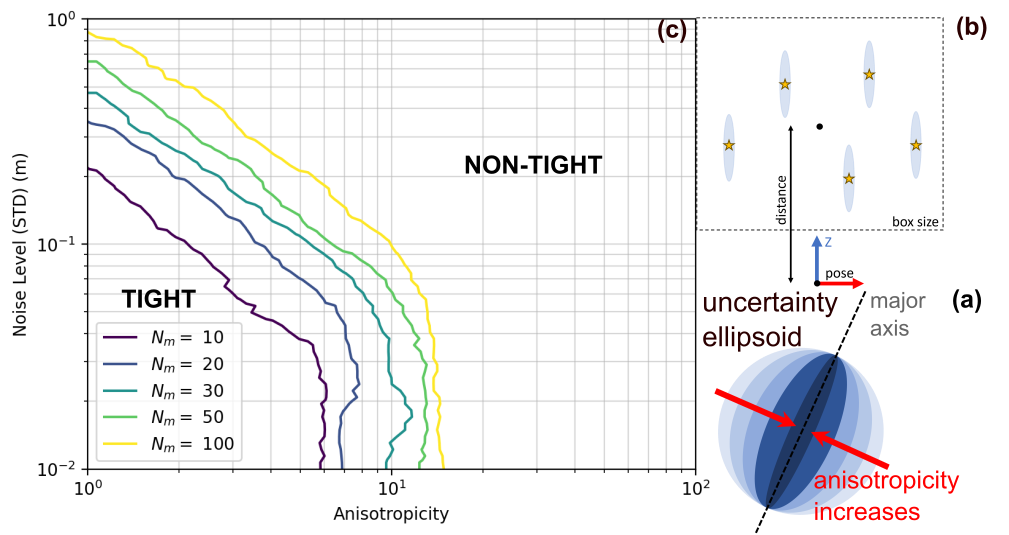
\includegraphics[width=\columnwidth]{figs/elliposoid_align_fig.png}
	%\vspace*{-0.3in}
	\caption{Investigation of the effect of anisotropicity on tightness of semidefinite relaxations for Wahba's problem. Landmark bounding box length was set to 1 m at an offset of 3 m. The boundary indicates where the minimum (smoothed) SVR exceeds $ 10^{6}$ across 30 trials (without redundant constraints). Subplot (a) shows how varying anisotropicity affects the uncertainty ellipsoid. Subplot (b) shows the problem setup, with ellipsoids aligned to the $z$-axis of the pose. Subplot (c) shows the tightness boundary for varying numbers of landmarks. Anisotropicity decreases the tightness boundary while increasing number of observed landmarks increases the boundary.}
	%\vspace*{-0.22in}
	\label{fig:ellipsoid_align}
\end{figure}

It is known that the tightness of SDP relaxations of least-squares perception problems depends on the level of noise in the measurements \cite{brialesConvexGlobal3D2017, rosenSESyncCertifiablyCorrect2019, cifuentesLocalStabilitySemidefinite2022}. For the case of rotational averaging, tightness of the relaxation has been linked to the magnitude of \textit{residual uncertainty} of pose estimates \cite{erikssonRotationAveragingStrong2018}. Here, we also observe that the \emph{orientation} of the uncertainty ellipsoids plays a key role in SDP tightness. This can be seen in Figure \ref{fig:wahba_axis_bnd}, in which two experiments are performed with respect to ellipsoid orientation: the random rotational perturbation of ellipsoid alignment and the `fanning out' of ray-aligned ellipsoids as the landmarks become more spread out (see diagrams in Figure \ref{fig:wahba_axis_bnd}).

\begin{figure}[!b]
	\centering
	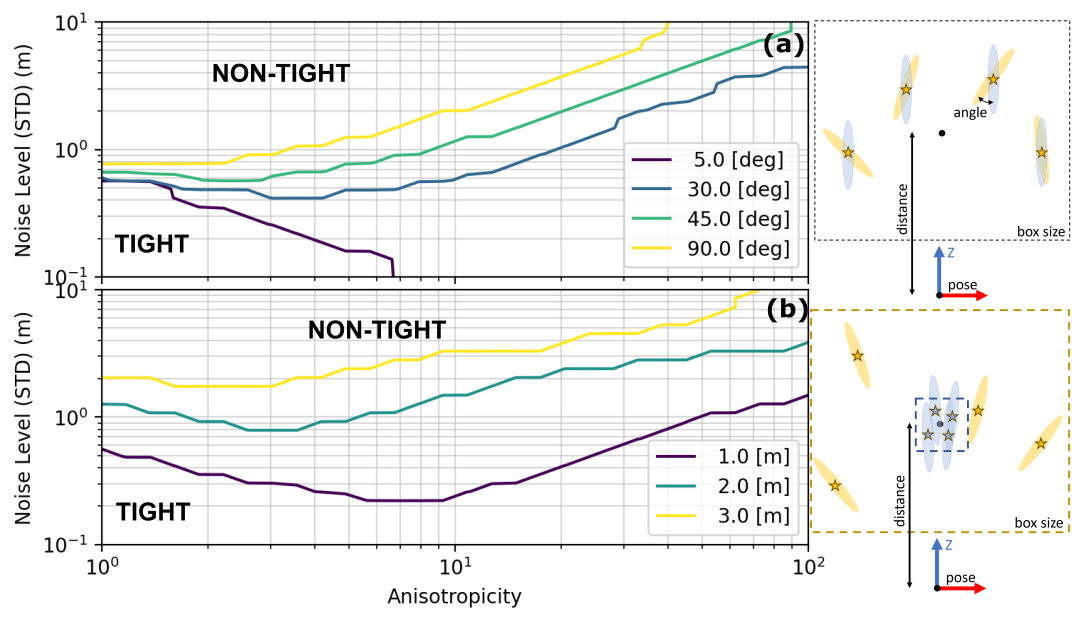
\includegraphics[width=\columnwidth]{figs/ellipsoid_study}
	\caption{Tightness boundary for Wahba's problem instance with 20 landmarks observed at 3 m and ellipsoidal noise model. The boundary indicates where the minimum (smoothed) SVR exceeds $ 10^{6}$ across 10 trials (without redundant constraints). In (a), axes of maximum uncertainty are aligned to pose $z$-axis then perturbed by random angles with different standard deviations (see legend). In (b), maximum uncertainty axis is aligned to pose-landmark ray and size of the bounding box on the landmarks is varied (size in legend). In both cases, increased variation of uncertainty ellipsoids eventually yields tighter relaxations as anisotropicity increases.}
	\label{fig:wahba_axis_bnd}
\end{figure}
In both cases, the same trend is observed: when the ellipsoids are \textit{aligned}, uncertainty is concentrated on a single axis and tightness is lost at a lower noise level. On the other hand, when the ellipsoids are highly \textit{misaligned}, uncertainty is not concentrated and the problems are tighter for much higher noise levels. 

These trends seem to indicate an inverse correlation between \emph{aggregate} or \emph{posterior} state-estimate uncertainty and the tightness of the SDP relaxation. This would explain why tightness appears to \emph{improve} with anisotropicity when the ellipoids are highly misaligned, since the aggregate uncertainty of the pose is still low. Exploration of a theoretical backing for this observation remains as future work.

\subsection{Study of Tightness in Stereo Problems}

We now turn our attention to a stereo-camera-based noise model. Both measurement noise level and the anisotropicity of the stereo-camera model depend strongly on the offset between a pose and the observed landmarks. In Figure \ref{fig:stereo_redun}, tightness boundaries are shown for localization problems in which the measurements and their associated covariances are drawn from the stereo-camera model with parameters matching the camera used for the dataset collection described in Section \ref{Sec:Dataset}. The figure shows results for localization with one pose and various numbers of landmarks. As expected, the level of noise for which the relaxation is tight is inversely proportional to the average distance between pose and landmarks. On the other hand, increasing the spread (bounding box) of the landmarks increases the tightness boundary, which is consistent with our previous observations for the ellipsoid model. Note that for this camera model, the single-pose problem is not very tight without redundant constraints \eqref{eqn:so3_constraints}, but becomes considerably tighter when the redundant constraints are employed.

In practical robotics scenarios, one way to reduce uncertainty is to observe the same landmarks from multiple poses (e.g., loop closure, visual-inertial odometry). In Figure \ref{fig:stereo_angle}, we consider the effect of adding a second pose that observes the landmarks from a different vantage point (same offset, but rotated by a given angle) with a relative-pose measurement between poses. Overall, uncertainty is reduced as long as additional information linking the different poses is introduced.\footnote{If there is no relative-pose measurement, then the localization problem is separable. Each separate instance is then subject to the same issue with alignment of measurement uncertainty.} Tightness boundaries are shown as the angle between the poses is increased to 90 deg with a noise level of 0.1 m and 0.1 rad on relative-pose measurements. Boundaries are also shown when the angle is fixed at 45 deg and the level of noise varies. In both cases, the results are consistent with the observations of Figure \ref{fig:wahba_axis_bnd}: tightness can be improved when observations \emph{collectively} reduce the uncertainty of the pose estimates.

\begin{figure}[!t]
	\centering
	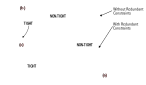
\includegraphics[width=\columnwidth]{figs/stereo_redun_study}
	\caption{Investigation of tightness boundaries for single-pose localization with a stereo-camera model (parameters in body text) when redundant constraints are considered. Boundaries indicate where the (smoothed) minimum SVR exceeds $ 10^{7}$ across 10 trials and a diagram of the scenario is shown in (a). (b) shows the effect of increasing the number of landmarks without redundant constraints. (c) shows the boundaries for the same model and scenario, but with redundant constraints included.}
	\label{fig:stereo_redun}
\end{figure}

\begin{figure}[!b]
	\centering
	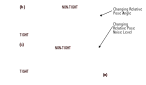
\includegraphics[width=\columnwidth]{figs/stereo_angle_study}
	\caption{Investigation of effect of pose interactions on tightness boundaries for two-pose localization with a stereo-camera model (parameters in body text). Boundaries indicates where the (smoothed) minimum SVR exceeds $ 10^{7}$ across 10 trials (without redundant constraints) and a diagram of the scenario is shown in (a). (b) shows the effect of observing the landmarks from a second pose at different vantage points, parameterized by the angle between poses. Noise level is fixed to 0.1 m and 0.1 rad. (c) Shows the effect of fixing the angle to 45 deg and varying the level of relative-pose noise (standard deviation in legend is equal for trans. and rot.).}
	\label{fig:stereo_angle}
\end{figure}

In Figure \ref{fig:stereo_slam_redun}, tightness boundaries are shown for the SLAM problem with redundant constraints using the same simulation setup as in Figure \ref{fig:stereo_redun}. We do not show the results for SLAM without redundant constraints because none of the cases that we studied were found to be tight. Again, increasing the number of landmarks expands the tightness boundary, but curiously, the spread of the landmarks (indicated by the bounding box) seems to have little-to-no effect on tightness. A study of a matrix-weighted SLAM problem with multiple poses is given in the next section.

\begin{figure}[!h]
	\centering
	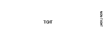
\includegraphics[width=\columnwidth]{figs/slam_lms_redun}
	\caption{Investigation of tightness boundaries for a single-pose SLAM problem with a stereo-camera model (parameters in body text) with redundant constraints. Boundaries indicates where the (smoothed) minimum SVR exceeds $ 10^{6}$ across 10 trials. A diagram of the scenario is shown in Figure \ref{fig:stereo_redun} (a). Boundaries are not shown when redundant constraints are not used because the problem was not tight across all of the parameters studied here.}
	\label{fig:stereo_slam_redun}
\end{figure}


\section{Dataset Results}\label{Sec:Dataset}

In this section, we test matrix-weighted localization and SLAM on the ``Starry Night'' dataset \cite{barfoot2011state}, which provides stereo-camera measurements of a set of known landmark locations (with known data association). The stereo camera has a baseline of 0.24 m, a focal length of 484.5 pixels and an assumed Gaussian noise model with a standard deviation of 6.32 pixels and 11.45 pixels for horizontal and vertical axes, respectively. At all times, the distance between the pose and the landmarks is within 1.75 m.

To assess tightness of stereo localization, we randomly select 30 poses from the dataset and solve the SDP relaxation with and without redundant constraints. We add relative-pose measurements between subsequent poses based on the ground-truth data and perturb these measurements by a controlled amount of (isotropic) noise allowing to assess the effect of these additional measurements. Figure \ref{fig:d3_loc_box} shows the effect of adding redundant constraints on the SVR (tightness) of the localization problem. When there are no restrictions on the pose selection (Figure \ref{fig:d3_loc_box}(a)), it is clear that adding redundant constraints is required to obtain tightness for reasonable noise levels. When poses are restricted so that they observe at least 15 landmarks each (Figure \ref{fig:d3_loc_box}(b)), we see that, without redundant constraints, the problem is tight for higher levels of relative-pose noise and, with redundant constraints, the problem is tight across \emph{all noise levels}. This is consistent with the observations in Section \ref{Sec:NoiseAnalysis}.

This experiment was also performed for matrix-weighted SLAM with 10 poses and the results are shown in Figure \ref{fig:d3_slam_box}. Without redundant constraints, the problem is not tight across the noise levels considered. On the other hand, with redundant constraints, the problem remains tight until the relative-pose measurement noise exceeds approximately 0.06 m and 0.06 rad, reflecting tightness up to a reasonable level of noise.  

\begin{figure}[!b]
	\centering
	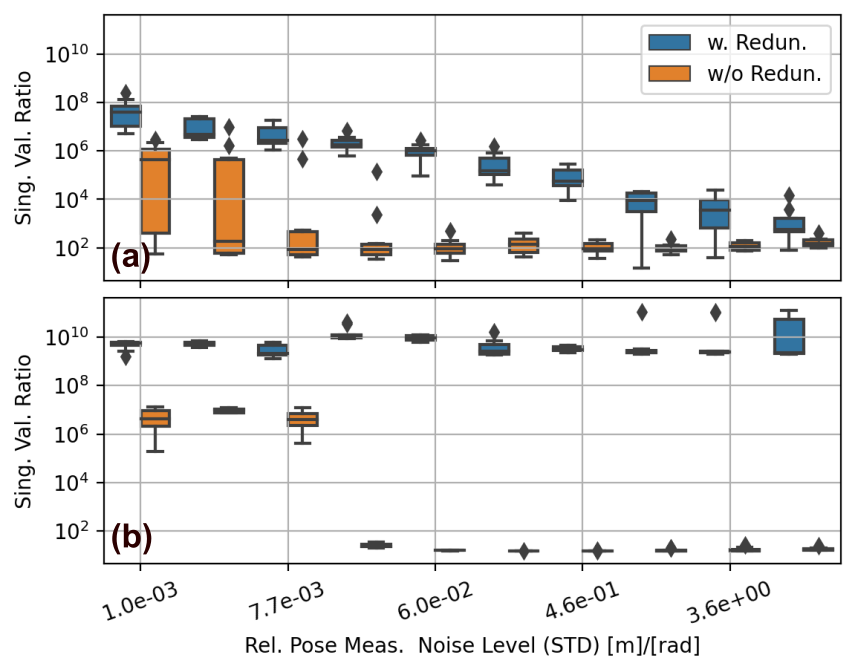
\includegraphics[width=\columnwidth]{figs/loc_box_plots}
	\caption{SVR results with and without redundant constraints for localization on random selections of 30 poses from the ``Starry Night'' dataset with relative-pose measurements between subsequent poses. 10 trials (random selection of poses) were performed at each noise level. (a) shows results when any pose can be selected, regardless of number of landmarks observed. (b) shows results when pose selection is restricted to poses that observe more than 15 landmarks.}
	\label{fig:d3_loc_box}
\end{figure}

\begin{figure}[!b]
	\centering
	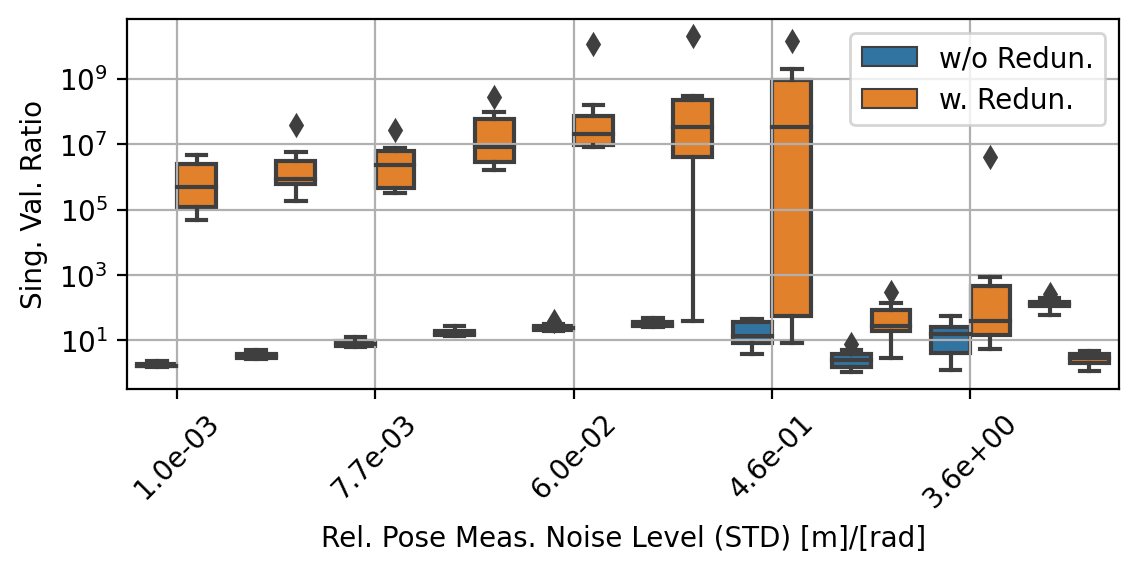
\includegraphics[width=\columnwidth]{figs/d3_slam_redun_box}
	\caption{SVR results with and without redundant constraints for SLAM on random selections of 10 poses from the ``Starry Night'' dataset with relative-pose measurements between subsequent poses. 10 trials (random selection of poses) were performed at each noise level. Without redundant constraints (blue), the SLAM problem is not tight for any of the tested noise levels. With redundant constraints (orange) the problem is tight for reasonable noise levels.}
	\label{fig:d3_slam_box}
\end{figure}

Figure \ref{fig:slam_local_min} shows an example of a local and global minimum for a 10-pose SLAM problem using measurements from the ``Starry Night'' dataset. Relative-pose measurements between subsequent poses were perturbed by Gaussian noise with standard deviation of $5.0 \times 10^{-2}$ m and $5.0 \times 10^{-2}$ rad in both rotation and translation. The local minimum was the result of running a Gauss-Newton (GN) solver from a randomly selected, poor initialization point while the global solution was found by solving the matrix-weighted SLAM SDP relaxation with redundant constraints.\footnote{Note that for good initializations, it was confirmed that the GN solver converged to the same cost and solution as the SDP relaxation.}

It is important to note that we have restricted these experiments to a low number of poses because of the \emph{necessary} addition of variables and constraints, which makes the matrix-weighted SLAM problem intractable for medium-to-large scale problems. However, we believe that the analysis and results presented herein are valuable to the robotics community and demonstrate that certifiable methods can be extended to this problem.

\section{Conclusions and Future Work}\label{Sec:Conclusions}

We have shown that inclusion of matrix weights in state-estimation problems can have profound implications on the tightness of their semidefinite relaxations. In the case of Wahba's problem and localization, matrix weights can decrease the noise level for which a given problem instance is tight to well below those found in practice. For SLAM, the introduction of matrix weights leads to a fundamental change in the formulation of the problem and the resulting formulation is not tight even for very low noise levels (without redundant constraints). These results stand in stark contrast to the same problems with scalar weights, which have tight relaxations for much higher noise levels.

We have explored the relationship between the shape of the noise distribution of measurements and its effect on tightness. Namely, anisotropicity in the underlying noise model results in nontight relaxations when uncertainty is concentrated in a given direction. This effect can be counteracted (to some extent) by increasing the number and variety of measurements in the problem.

We have shown that the `tightness boundary' can be improved by adding specific redundant constraints to the problem. These constraints can recover tight semidefinite relaxations for noise levels that are commonly found in practice. We have also shown that tightness can be achieved with specific variable and constraint selections, without resorting to the full Lasserre-moment hierarchy. 
%We plan to continue to explore methods to generalize this parsimonious selection of tightening constraints and variables for other robotics and state-estimation problems.

However, the use of redundant constraints still precludes the application of the fast, low-rank-exploiting methods described in Section \ref{Sec:FastPerception}. The significance of this preclusion cannot be understated. At present, it represents the dividing line between those robotics problems that can be solved globally in real time and those that must be solved offline. Exploration of amendments to the \emph{Riemannian Staircase} and \emph{Burer-Monteiro} techniques to accommodate redundant constraints is an exciting avenue of future work. 

In a similar vein, it is our hope that the empirical relationships highlighted herein will inspire new theoretical methods to determine \emph{a priori} whether a given problem instance has a tight relaxation (without redundant constraints)\cite{carloneEstimationContractsOutlierRobust2022}. Such a result would be crucial in assessing whether a problem can be solved or certified in real time. 

\section{Acknowledgments}

The authors would like to thank National Sciences and Engineering Research Council of Canada (NSERC) for their generous support of this work. The authors would also like to thank Matt Giamou and Dave Rosen for their useful insights and suggestions.
 
\bibliographystyle{IEEEtrans}
\bibliography{MatrixWeightCert,RedundantConstraints,Software}

%\renewcommand\appendixname{Appendix (arXiv Only)}
%\appendix
\section{Supplementary Material}

%\numberwithin{equation}{section}
%\renewcommand{\theequation}{\thesection.\arabic{equation}}

\subsection{Stereo-Camera Model}\label{SM:stereo}

In this section, we seek to convert pixel measurements from left- and right-rectified stereo images to Euclidean point measurements. We also seek to determine an appropriate model of the uncertainty of the measurement in the Euclidean space. We assume that left and right stereo frames have their $z$-axes aligned with the viewing direction and their other axes coincident. We also assume that they are separated by baseline distance $ b\in \mathbb{R} $ and that the camera frame is coincident with the left camera.  

Consider a 3D point expressed in the world frame, $ \bm{x}_w = \begin{bmatrix} x_w & y_w & z_w  \end{bmatrix}^T $ representing a feature that we wish to track. This point can be expressed in the left camera frame as  $ \bm{x}_c = \bm{C}_{cw} \bm{x}_w + \bm{t}^{wc}_c $, where $ \bm{C}_{cw} \in \mbox{SO}(3)$ is the rotation matrix from the world to the camera frame and $ \bm{t}^{wc}_c \in \mathbb{R}^3 $ is vector from the world frame origin to the camera frame origin expressed in the camera frame.

Assuming a pinhole stereo-camera, the resulting pixel measurements can be expressed as follows:
\begin{equation}
	\begin{bmatrix}
		p_{ul}\\p_{vl}\\p_{ur}\\p_{vr}
	\end{bmatrix} = \frac{1}{z_c}\begin{bmatrix}
		f_{u} & 0 & c_{u} & 0\\
		0 & f_{v} & c_{v} & 0\\
		f_{u} & 0 & c_{u} & -b f_{u}\\
		0 & f_{v} & c_{v} & 0
	\end{bmatrix} \begin{bmatrix}
	\bm{x}_c \\ 1
	\end{bmatrix} + \bm{\epsilon}_{p},
\end{equation}
where $ u $ and $ v $ subscripts represent horizontal and vertical pixel directions, respectively, $ l $ and $ r $ subscripts represent left and right cameras, respectively, $ p_{ij} $ represents the pixel measurement, $ f_{i} $ represents the focal length parameter, and $ c_{i} $ represents the camera centre parameter for direction $ i $ of camera $ j $. The variable $ \bm{\epsilon}_{p} $ represents noise on the pixel measurements and is assumed to have zero-mean, Gaussian distribution,
$ \bm{\epsilon}_{p} \sim \mathcal{N}(\bm{0}, \bm{\Sigma}_p) $,
with covariance matrix $ \bm{\Sigma}_p = \diag{\sigma_u^2 ,\sigma_v^2,\sigma_u^2, \sigma_v^2} $, where $ \sigma_i $ represents the standard deviation of the noise. 

We define the \textit{disparity}, $ d $, of a given feature as the horizontal difference between the feature's position in the right and left images in terms of pixels: $ d = p_{ul} - p_{ur} $. We define the intermediate, Gaussian-distributed measurement, 
\begin{equation}
	\bm{y} = \begin{bmatrix}p_{ul}&p_{vl}&d\end{bmatrix}^T \sim \mathcal{N}(\bm{\mu}_y, \bm{\Sigma}_y),
\end{equation}
where the mean and covariance matrices are given by
\begin{equation}
	\bm{\mu}_y = \begin{bmatrix}
		\frac{1}{z_c}f_u x_c + c_u \\ \frac{1}{z_c}f_v y_c + c_v \\ \frac{1}{z_c}f_u b
	\end{bmatrix},\quad \bm{\Sigma}_y = \begin{bmatrix}
		\sigma_u^2 & 0 & \sigma_u^2\\
		0 & \sigma_v^2 & 0 \\
		\sigma_u^2 & 0 & 2\sigma_u^2
	\end{bmatrix}.
\end{equation}
Given this measurement, we can use the (known) intrinsic camera parameters to generate Euclidean \textit{pseudo-measurements}, $ \hat{\bm{x}} = \begin{bmatrix}\hat{x}_c &\hat{y}_c & \hat{z}_c \end{bmatrix}^T $, of the (unknown) feature locations via the following mapping:
\begin{equation}
	\bm{g}^{-1}:~(\mathbb{R}^2\times\mathbb{R}_+) \rightarrow \mathbb{R}^3, \quad \mbox{s.t.}~\hat{\bm{x}} = \bm{g}^{-1}(\bm{y})=b\begin{bmatrix}
	 	\frac{p_{ul}-c_u}{d} \\ \frac{p_{vl}-c_v}{d} \\ \frac{f_u}{d} 
	 \end{bmatrix}.
\end{equation}
Although this transformation is clearly nonlinear, we make the assumption that the distribution of $ \hat{\bm{x}} $ remains Gaussian. To approximate the covariance of the pseudo-measurement, we map the intermediate measurement covariance through the linearized Jacobian of this transformation:
\begin{equation}
	\bm{G} = \frac{\partial \bm{g}^{-1}(\bm{y})}{\partial \bm{y}} = b\begin{bmatrix}
		\frac{1}{d} & 0 & -\frac{p_{ul} - c_u}{d^2} \\
		0 & \frac{f_u}{f_v d} & -\frac{f_u}{f_v }\frac{(p_{vl} - c_v)}{d^2} \\
		0 & 0 & -\frac{f_u}{d^2}
	\end{bmatrix}.
\end{equation}
Typically, such a linearization is performed about a prior belief -- as in a Kalman filter -- or previous iterate -- as in iteratively re-weighted least squares --  of the variables involved. However, in the global-optimization context, neither of these options are available and we choose to linearize about the measurement itself. 

Therefore, the noise model of the pseudo-measurement can be expressed as
\begin{equation}
	 \hat{\bm{x}} = \bm{x}_c + \bm{\epsilon}_x, ~ \bm{\epsilon}_x \sim \mathcal{N}(\bm{0}, \bm{\Sigma}_x),
\end{equation}
where $ \bm{\epsilon}_x $ represents an approximately Gaussian-distributed variable with zero mean and covariance given by $ \bm{\Sigma}_x = \bm{G}\bm{\Sigma}_y \bm{G}^T $.

It is instructive to consider the following alternate formulation of the Jacobian:
\begin{equation}
	\bm{G} =\hat{z}_c\begin{bmatrix}
		\frac{1}{f_u} & 0 & -\frac{\hat{x}_c}{f_u b } \\
		0 & \frac{1}{f_v } & -\frac{\hat{y}_c}{f_u b } \\
		0 & 0 & -\frac{\hat{z}_c}{f_u b}
	\end{bmatrix}.
\end{equation}
We see that the Jacobian matrix scales linearly with the $z$-axis coordinate, $\hat{z}_c$, meaning that the variance of the Euclidean measurement scales quadratically with this variable. Ignoring the off-diagonal terms, we note that the anistropicity of the measurement is approximately proportional to $\frac{\hat{z}_c}{b}$.

\subsection{SDP Stability of Matrix-Weighted Localization}\label{SM:SDPStability}

In this section, we prove that Problem \eqref{opt:Localize} enjoys the property of `SDP stability' established in \cite{cifuentesLocalStabilitySemidefinite2022}. That is, the convex relaxation of Problem \eqref{opt:Localize} is tight whenever the set of measurements has sufficiently low noise. In particular, we connect the SDP stability to the well-known condition that the observed landmarks are not coplanar, which has been shown to lead to a unique solution for point-set regression \cite{arunLeastSquaresFittingTwo1987}. Such results have been given for other state-estimation problems \cite{rosenSESyncCertifiablyCorrect2019, tianDistributedCertifiablyCorrect2021} and our proof closely follows the development given in \cite{wiseCertifiablyOptimalMonocular2020}.

\begin{definition}[Noise-free Measurements]
	Given the setting of Problem \eqref{opt:Localize}, we define the set of \emph{noise-free measurements} for a given set of poses, $\left\{(\bar{\bm{C}}_{i0}, \bar{\bm{t}}_i^{i0}) ~ \forall i \in \VertSetP \right\}$, as
	\begin{equation}
		\left\{\bar{\bm{m}}_i^{ki} = \bar{\bm{C}}_{i0} \bm{m}_0^{k0} - \bar{\bm{t}}_i^{i0},~ \forall (i,k)\in \EdgeSet_m\right\},
	\end{equation}
	and collect all such measurements in a vector, $\bar{\bm{m}}$.
\end{definition}

\begin{theorem}[SDP-Stability of Matrix-Weighted Localization]
Consider the setting of Problem \eqref{opt:Localize} with positive definite weighting matrices ($ \bm{W}_{ik} \succ 0$) and suppose the set of landmarks observed from a given pose are not coplanar. Let $\tilde{\bm{m}}$ be a vector containing all of the pose-landmark measurements for the problem and let $\bar{\bm{m}}$ be the set of noise-free measurements associated with the globally optimal solution of the problem with the same ordering as $\tilde{\bm{m}}$. Then, there exists some $\epsilon > 0$ such that if $\Vert \tilde{\bm{m}} - \bar{\bm{m}} \Vert^2 < \epsilon $, the SDP relaxation of the problem is tight (strong duality holds) and the global minimizer can be recovered from the SDP solution.
\end{theorem}
\begin{proof}
To prove the theorem, we show that the conditions of Theorem 3.9 from \cite{cifuentesLocalStabilitySemidefinite2022} are satisfied when the assumptions of our theorem hold. In the following, we treat the measurements, $\tilde{\bm{m}}$, as a set of \emph{parameters} on which the cost of the problem depends. Since there are no relative-pose measurements in Problem \eqref{opt:Localize}, it is separable and we can prove the result for a single-pose problem (fixed pose $i$) without loss of generality.
The conditions of Theorem 3.9 are as follows:
\begin{enumerate}
	\item The cost and constraints are quadratic in the variables. \label{thm1:cond1}
	\item The cost depends continuously on the set of parameters, $\tilde{\bm{m}}$. \label{thm1:cond2}
	\item When constructed with $\bar{\bm{m}}$ rather than $\tilde{\bm{m}}$, the cost becomes \emph{strictly convex}, with the same unconstrained minimum as the original problem.\label{thm1:cond3}
	\item The Abadie Constraint Qualification (ACQ) holds for the feasible set at the global solution. \label{thm1:cond4}
\end{enumerate}
Let $\bm{y} = \begin{bmatrix}\vect{\bm{C}_{i0}}^T & \bm{t}_i^{i0^T} \end{bmatrix}^T \in\mathbb{R}^{12}$ be the vectorized form of the variables.
The cost function for pose $i$ in Problem \eqref{opt:Localize} is given by 
\begin{equation}\label{eqn:LocCost}
	f_i(\tilde{\bm{m}},\bm{y}) = \sum\limits_{(i,k)\in\EdgeSet_m} \bm{e}_{ik}^T \bm{W}_{ik} \bm{e}_{ik}.
\end{equation}
We can write $\bm{e}_{ik}$ as an affine function of $\bm{y}$
\begin{equation}
	\bm{e}_{ik} = \tilde{\bm{m}}_i^{ki} - \bm{A}_k \bm{y}, ~\forall ~(i,k)\in \EdgeSet_m,
\end{equation}
where $\bm{A}_k = \begin{bmatrix} \bm{m}_0^{k0^T}\otimes\bm{I}& -\bm{I} \end{bmatrix}\in\mathbb{R}^{3\times12}$. The cost function becomes 
\begin{equation}
	f_i(\tilde{\bm{m}},\bm{y}) = \bm{y}^T \bm{Q} \bm{y} + \bm{b}^T \bm{y} + c, 
\end{equation}
where
\begin{gather}
	\bm{Q} = \sum\limits_{(i,k)\in\EdgeSet_m} \bm{A}_k^T \bm{W}_{ik} \bm{A}_k, \\
	\bm{b} = -2\sum\limits_{(i,k)\in\EdgeSet_m} \bm{W}_{ik}\tilde{\bm{m}}_i^{ik}, \\
	c=\sum\limits_{(i,k)\in\EdgeSet_m} \tilde{\bm{m}}_i^{ik^T}\bm{W}_{ik}\tilde{\bm{m}}_i^{ik}.
\end{gather}
We see immediately that the cost function depends quadratically on the variables, $\bm{y}$, and quadratically (thus continuously) on the parameters, $\tilde{\bm{m}}$. Together with the fact that the $\mbox{O}(3)$ constraints are quadratic, conditions \ref{thm1:cond1}) and \ref{thm1:cond2}) are satisfied.

Now, let $\bar{\bm{y}}$ represent the vectorized form of the global solution and consider the cost function, $f_i(\bar{\bm{m}},\bm{y})$, constructed using the noise-free measurements, $\bar{\bm{m}}$, associated with the global solution. Since $f_i(\bar{\bm{m}},\bm{y})$ is a sum of quadratic forms, we have that $f_i(\bar{\bm{m}},\bm{y})\geq 0$. Moreover, its global minimizer is $\bar{\bm{y}} $ since $f_i(\bar{\bm{m}},\bar{\bm{y}})= 0$. 

To conclude that this minimizer is unique, we must show \emph{strict} convexity of $f_i(\bar{\bm{m}},\bm{y})$, which is implied if $\nabla_{\bm{y}}^2 f_i(\bar{\bm{m}},\bm{y}) = \bm{Q} $ is strictly positive definite \cite{boydConvexOptimization2004}. Note that since the weights are positive definite ($\bm{W}_{ik}\succ 0 $) we already have that $\bm{Q} \succeq 0$. To show positive definiteness, it remains to show that $\bm{Q}$ is full-rank. To this end, note that we can write
\begin{equation}
	\bm{Q} = \bm{A}^T \bm{W} \bm{A},
\end{equation}
where
\begin{gather}
	\bm{W} = \diag{\bm{W}_{i1},\ldots,\bm{W}_{iN}},\\
	\bm{A} = \begin{bmatrix}
		 \bm{A}_1 \\ \vdots \\ \bm{A}_N
	\end{bmatrix} = \begin{bmatrix}
		 \bm{m}_0^{10^T} & 1 \\
		 \vdots& \vdots\\
		 \bm{m}_0^{N0^T} & 1
	\end{bmatrix}\otimes \bm{I}_3,
\end{gather}
and we have re-indexed the landmarks from $1$ to $N$ for convenience. We also define
\begin{equation*}
	\bm{B} = \begin{bmatrix}
		\bm{m}_0^{10^T} & 1 \\
		\vdots&\vdots\\
		\bm{m}_0^{N0^T} & 1
	\end{bmatrix}.
\end{equation*}
Since $\bm{W}$ is full rank, we are required to show that $\rank{\bm{A}} = 12$. 
Recall that the spectrum of a Kronecker product, $\bm{A}\otimes\bm{B}$, is given by $\left\{ \mu\lambda,~ \forall \mu \in \sigma(\bm{A}),~ \lambda \in \sigma(\bm{B})\right\}$, where $\sigma()$ denotes the spectrum of eigenvalues.
Therefore, $\rank{\bm{A}} = 12$ is equivalent to the fact that $\rank{\bm{B}}=4$. We can subtract the first row from the remaining rows of $\bm{B}$ without changing its row rank. Thus,
\begin{equation*}
	\rank{\bm{B}} = \rank{\begin{bmatrix}
			\bm{m}_0^{10^T} & 1 \\
			\bm{D} & \bm{0}
		\end{bmatrix}}, ~ \bm{D} = \begin{bmatrix}
		(\bm{m}_0^{20}-\bm{m}_0^{10})^T  \\
		\vdots\\
		(\bm{m}_0^{N0}-\bm{m}_0^{10})^T 
	\end{bmatrix}.\\	
\end{equation*}
Since the landmarks are not coplanar by assumption, $\rank{\bm{D}}=3$ and, since $\rank{\bm{B}} = \rank{\bm{D}} + 1$, condition \ref{thm1:cond3}) holds.
 
Finally, the ACQ holds at any feasible point by the fact that $\mbox{O}(3)$ defines a radical ideal (c.f. \cite{wiseCertifiablyOptimalMonocular2020,cifuentesLocalStabilitySemidefinite2022}), giving the final condition of Theorem 3.9.
\end{proof}

We conclude this section with two remarks. First, the assumption that the weight matrices are positive definite (i.e., not degenerate) is not strictly required as long as $\rank{\bm{A}^T \bm{W} \bm{A}}=12$ is guaranteed by sufficient measurements. As mentioned above, degenerate weight matrices were encountered in \cite{brialesConvexGlobal3D2017} when measurements of lines and planes were considered. Second, the extension of this proof to include relative-pose measurements should be straightforward since it has already been proved when \emph{only} relative-pose measurements are considered (at least for the case of a weakly connected measurement graph) \cite{rosenSESyncCertifiablyCorrect2019}.

\subsection{Tightness Boundary Smoothing}\label{SM:Smoothing}

As mentioned in the main-body text, we plot tightness boundaries based on the parameters for which the minimum SVR across all trials passes a threshold. However, it was initially found that the resulting contour plots were quite noisy and difficult to interpret even when the number of trials was increased considerably. To filter the data, the median of minimum SVR values was taken over an $N$-by-$N$ block in the parameter space (centered on a given parameter value) and the result was used to generate the smoothed contours. It was found that $N=7$ was sufficient to ensure adequate smoothing. For all plots, the parameter space was sampled using a $70$-by-$70$ grid. A comparison of the contours on the raw minimum SVR data versus the filtered data is shown in Figure \ref{fig:filter}, in which the data corresponds to the data in Figure \ref{fig:ellipsoid_align} in the main text. 
\begin{figure}[!ht]
	\centering
	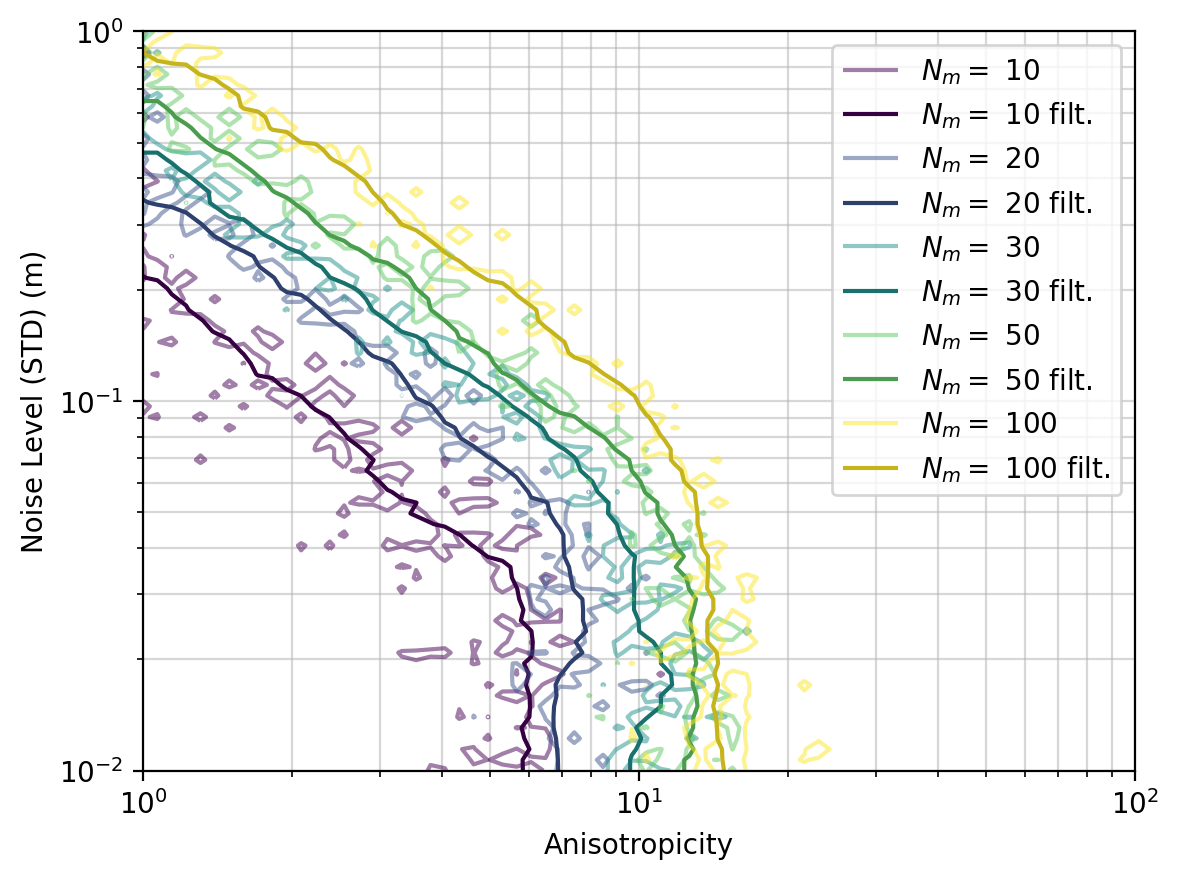
\includegraphics[width=\columnwidth]{figs/filter_compare}
	\caption{Comparison of tightness boundary contours with and without median filter for the results in Figure \ref{fig:ellipsoid_align}. Darker contours (marked ``filt.'' in legend) represent the smoothed contours that were used in the body text.}
	\label{fig:filter}
\end{figure}

\vfill

\end{document}


